\documentclass[12pt,oneside]{report}
\usepackage{makecell ,tabularx}
\usepackage{cellspace}
\usepackage[utf8]{inputenc}
\usepackage[T1]{fontenc}
\usepackage[english]{babel}
\usepackage{titlepic}
\usepackage{graphicx}
\usepackage[11pt]{moresize}
\usepackage{eso-pic}
\usepackage[export]{adjustbox}
\usepackage{fancyhdr}
\usepackage{vmargin}
\usepackage{titlesec}
\usepackage{textpos}
\usepackage{minted}
\usepackage{float}
\usepackage[breaklinks=true,hidelinks]{hyperref}
\usepackage[Lenny]{fncychap}
\usepackage{titlesec, blindtext, color}
\usepackage{listings}
\usepackage{xcolor}
\usemintedstyle{manni}

\definecolor{gray75}{gray}{0.75}
\newcommand{\hsp}{\hspace{20pt}}

\renewcommand{\thesection}{\arabic{section}}
\renewcommand{\thefigure}{\arabic{chapter}.\arabic{section}.\arabic{figure}}

%%%% JSON settings %%%%%%%%%%%%%%
\colorlet{punct}{red!60!black}
\definecolor{background}{HTML}{EEEEEE}
\definecolor{delim}{RGB}{20,105,176}
\colorlet{numb}{magenta!60!black}

\lstdefinelanguage{json}{
    basicstyle=\normalfont\ttfamily,
    numbers=left,
    numberstyle=\scriptsize,
    stepnumber=1,
    numbersep=3pt,
    showstringspaces=false,
    breaklines=true,
    frame=lines,
    backgroundcolor=\color{background},
    literate=
     *{0}{{{\color{numb}0}}}{1}
      {1}{{{\color{numb}1}}}{1}
      {2}{{{\color{numb}2}}}{1}
      {3}{{{\color{numb}3}}}{1}
      {4}{{{\color{numb}4}}}{1}
      {5}{{{\color{numb}5}}}{1}
      {6}{{{\color{numb}6}}}{1}
      {7}{{{\color{numb}7}}}{1}
      {8}{{{\color{numb}8}}}{1}
      {9}{{{\color{numb}9}}}{1}
      {:}{{{\color{punct}{:}}}}{1}
      {,}{{{\color{punct}{,}}}}{1}
      {\{}{{{\color{delim}{\{}}}}{1}
      {\}}{{{\color{delim}{\}}}}}{1}
      {[}{{{\color{delim}{[}}}}{1}
      {]}{{{\color{delim}{]}}}}{1},
}

%%%% TabularX settings %%%%%%%%%%%%%%

\setcellgapes{12pt}
\newcolumntype{Y}{>{\centering\arraybackslash}X}
\setlength\cellspacetoplimit{12pt}
\setlength\cellspacebottomlimit{12pt}
\newcolumntype{T}[1]{>{\centering\arraybackslash}m{#1}}
\newcolumntype{S}[1]{>{\centering\arraybackslash\footnotesize}m{#1}}
\newcolumntype{R}[1]{>{\small\arraybackslash}m{#1}}

%%%% Footer and Header %%%%%%%%%%%%%%

\pagestyle{fancy}
\fancyhf{}
\fancyfoot[C]{}
\fancyfoot[R]{Page -- \thepage}
\renewcommand{\footrulewidth}{0.5pt}
\renewcommand{\headrulewidth}{0pt}


% Redefine the plain page style
\fancypagestyle{plain}{
\fancyhf{}
\fancyfoot[C]{\footnotesize{\rightmark}}
\fancyfoot[R]{Page -- \thepage}
\renewcommand{\footrulewidth}{0.5pt}
\renewcommand{\headrulewidth}{0pt}
}

\begin{document}
%----------------------------------------------------------------------------------------
%	MARGINS
%----------------------------------------------------------------------------------------
\setmarginsrb{ 1.2in}   % left margin
             { 0.6in}   % top margin
             { 1.2in}   % right margin
             { 0.8in}   % bottom margin
             {  20pt}   % head height
             {0.25in}   % head sep
             { 9pt}     % foot height
             { 0.75in}  % foot sep

%%%%%%% Title Page %%%%%%%%%%%%%%%%%%%

%---title format---
%%%%%%%%%%%%%%%%%%%%%%%%%%%%%%%%%%%

\titleformat{\chapter}[hang]{\Huge\bfseries}{\thechapter\hsp\textcolor{gray75}{|}\hsp}{0pt}{\Huge\bfseries}
%%%%%%%%%%%%%%%%%%%%%%%%%%%%%%%%%%%%

	\begin{titlepage}
		\begin{center}
			\vspace*{\fill}
			
 			\begin{figure}[h]
       	 		
\includegraphics[width=5cm, center]{Figures/Logo_ECAM.jpg}	
       	 	\end{figure}
 			\vspace{\baselineskip}
 			
       		\HUGE{Web architechture}
       		\vspace{0.5cm}


       		\normalsize{Décembre 2019 \\} 
			
       		\vspace*{\fill}
       		
       		\large{SMITS Victor 16107}
            \vspace{\baselineskip}
            
            \large{Ecole centrale des arts et métiers}
            \vspace{\baselineskip}
            
       		\small{MIN1}
       		\vspace{\baselineskip}
       		
       		\normalsize{Année académique 2019-2020}
   		\end{center}
	\end{titlepage}

%%%%% table of content %%%%%%
\tableofcontents

%%%%% Documents %%%%%%
\chapter{Spécification}
\label{chap:Spécification}

	\vspace{\baselineskip}
	
\section{Objectif du site}
	\paragraph{}
		Le site doit permettre à des personnes de s’inscrire et se désinscrire de leur groupe à des session de sport. 
		
		
\section{Acteur}
	\paragraph{}
		\begin{itemize}
			\item Utilisateur : personne qui utilise le site et s'inscrivant à des session de sport
			\item Administrateur : personne administrant le site et ayant tout contrôle sur les sessions de sport organisé
		\end{itemize}
		

\section{User Stories}
	\begin{center}
		\begin{tabularx}{\linewidth}{| Y | T{0.15\linewidth} |}
			\hline
			User Stories & Priority \\
			\hline
			En tant qu’utilisateur, je dois pouvoir me créer un compte sur le site & 2 \\
			\hline
			En tant qu'utilisateur, je dois pouvoir sélectionner le mois et l'année pour afficher les sessions qui m'intéresse & 2 \\
			\hline
			En tant qu’utilisateur, je dois pouvoir m’inscrire à une session de sport un certain jour & 1 \\
			\hline
			En tant qu’utilisateur, je dois pouvoir être inscrit automatiquement à une session & 1 \\
			\hline
			En tant qu’utilisateur, je dois pouvoir me désinscrire à une session & 1 \\
			\hline
			En tant qu’utilisateur, je dois pouvoir voir qui est inscrit pour chaque session & 2 \\
			\hline

		\end{tabularx}
	\end{center}
	
	\begin{center}
		\begin{tabularx}{\linewidth}{| Y | T{0.15\linewidth} |}
			\hline
			En tant qu’utilisateur, je veux pouvoir voir dynamiquement le nombre de séance qui reste dans mon abonnement & 2\\
			\hline
			En tant qu'utilisateur, je veux pouvoir modifier mon profile & 1\\
			\hline
			En tant qu'utilisateur, je veux pouvoir m'inscrire a une session uniquement si il me reste des abonnements a disposition. & 2\\
			\hline
			En tant qu’administrateur, je dois pouvoir annuler une session & 2 \\
			\hline
			En tant qu'administrateur, je dois pouvoir créer un type de session & 2 \\
			\hline
			En tant qu'administrateur, je dois pouvoir générer les sessions pour un nombre d'année & 1 \\
			\hline
			En tant qu'administrateur, je dois pouvoir gérer les abonnement des utilisateurs & 2 \\
			\hline
			En tant qu'administrateur, je veux pouvoir supprimer un utilisateur du système & 1\\
			\hline
			En tant qu'administrateur, je dois pouvoir créer une nouvelle session peut importe la date & 2\\
			\hline
			En tant qu'administrateur, je veux pouvoir gérer les types de sessions disponible pour l'inscription automatique & 2\\
			\hline
			En tant qu'administrateur, je veux pouvoir modifier un type de session & 1\\
			\hline
			En tant qu'administrateur, je veux pouvoir supprimer un type de session & 1\\
			\hline
		\end{tabularx}
	\end{center}

\vspace{\baselineskip}
\section{Contrainte non fonctionnelles}
	\paragraph{}
		\begin{itemize}
			\item Le site dois être user-friendly pour des personnes non adepte de la technologie. 
			\item Le site doit être responsive afin de pouvoir l'utiliser sur tout type de d'écran. 
		\end{itemize}

\newpage
\section{Mockup}
	\subsection{Login}
		\begin{figure}[!htbp]
       	 	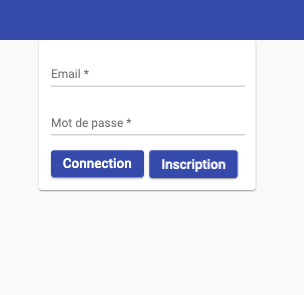
\includegraphics[width=0.5\linewidth, center]{Mockup/Login.png}
       	 	\caption{Page de connection}
       	\end{figure}
       	
    \vspace{\baselineskip}
	\subsection{Accueil}
		\begin{figure}[!htbp]
       	 	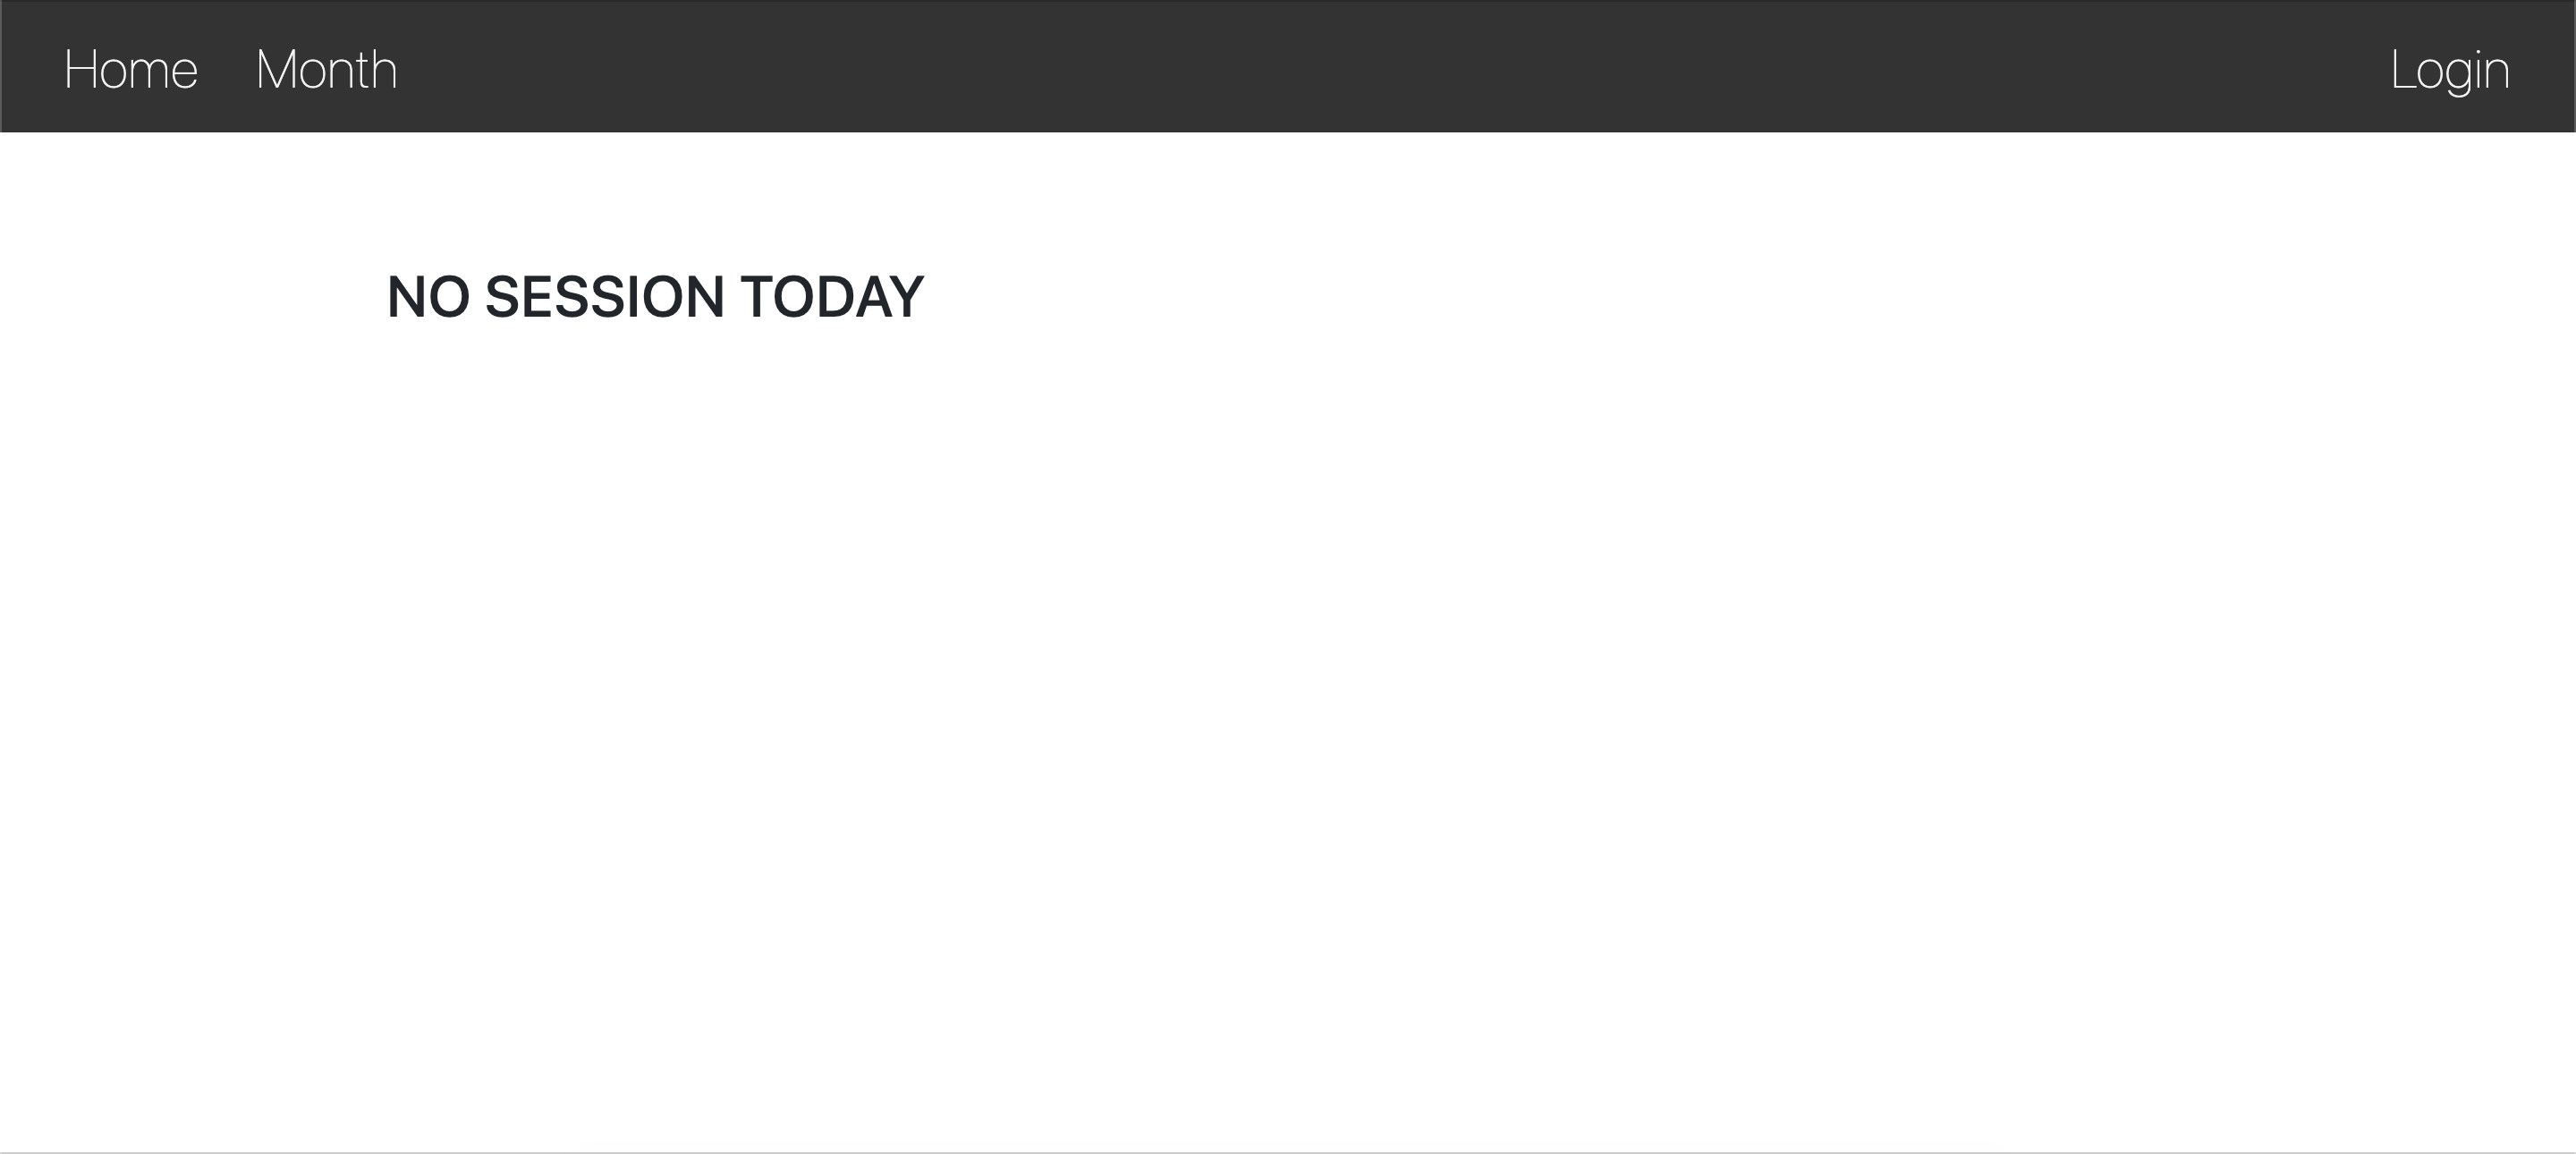
\includegraphics[width=0.8\linewidth, center]{Mockup/Accueil.png}
       	 	\caption{Page d'accueil}
       	\end{figure}
       	
       	
	\newpage
	\subsection{Inscription}
		\begin{figure}[!htbp]
       	 	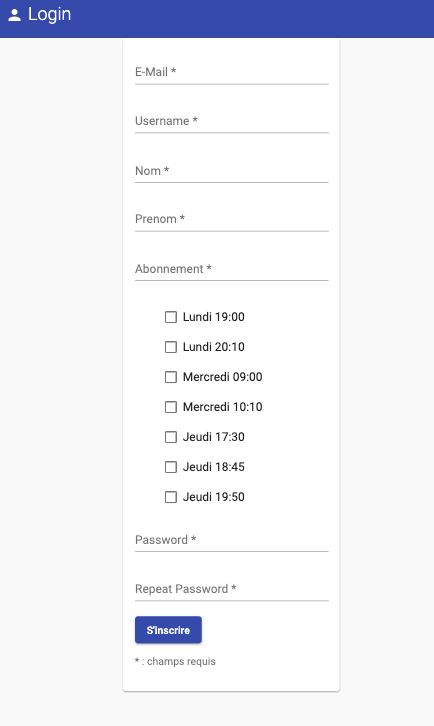
\includegraphics[width=0.5\linewidth, center]{Mockup/Inscription.png}
       	 	\caption{Page d'inscription au site}
       	\end{figure}
    
       
       
	\newpage
	\subsection{Month}
		\begin{figure}[h!]
       	 	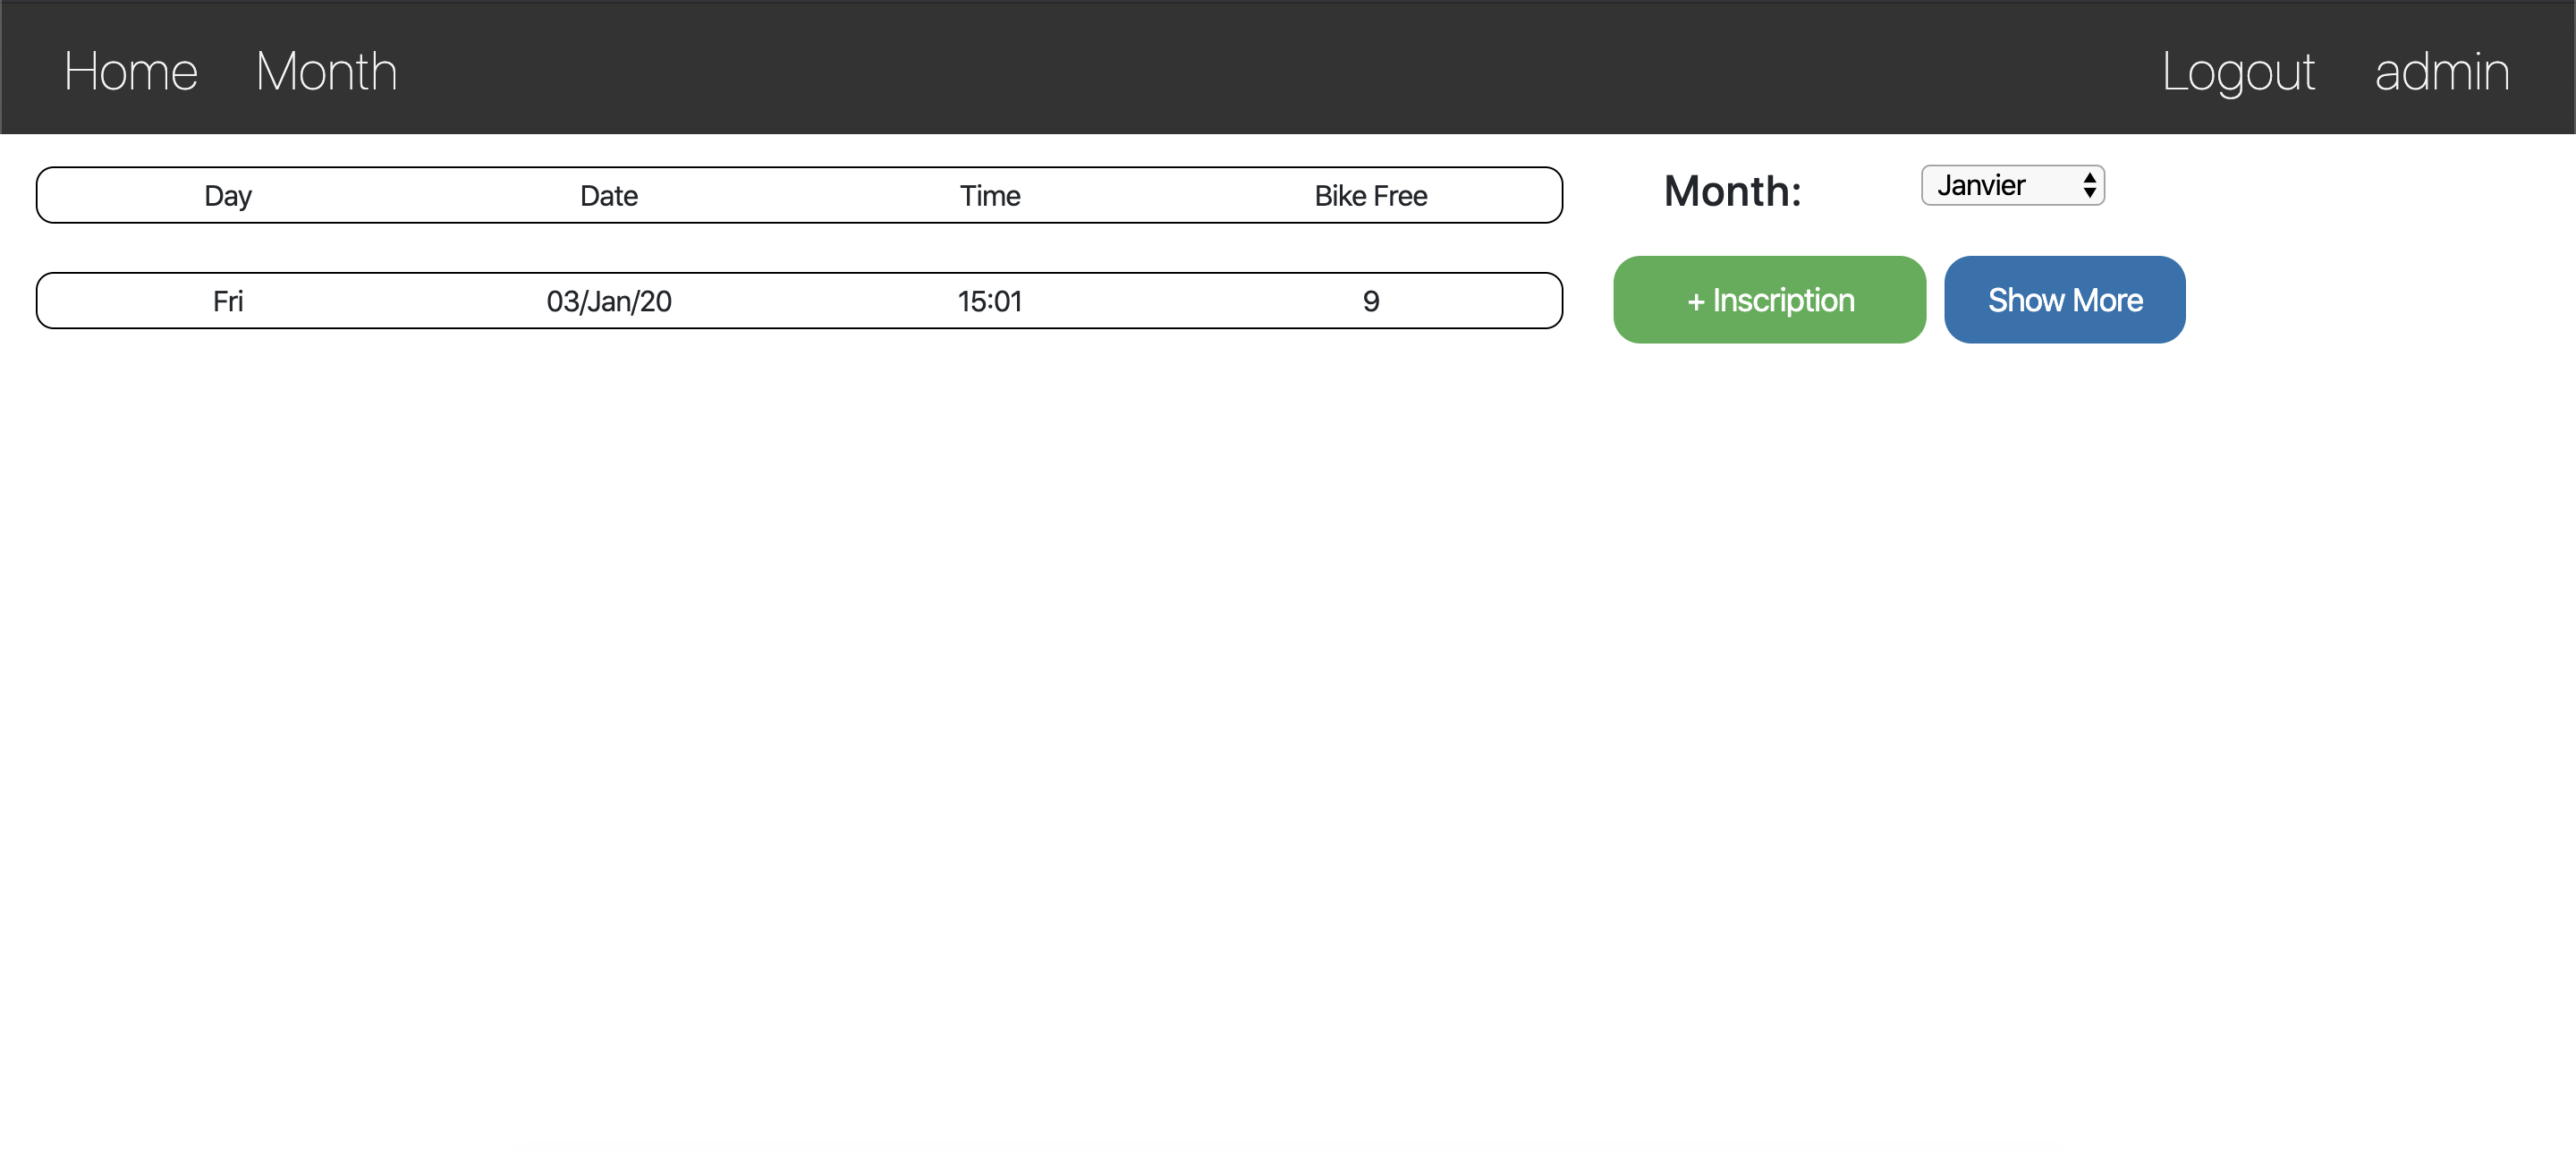
\includegraphics[width=0.8\linewidth, center]{Mockup/Month.png}
       	 	\caption{Page d'affichage des sessions du mois}
       	\end{figure}
       	

	\vspace{\baselineskip}	
	\subsection{Admin - Session}
		\begin{figure}[h!]
       	 	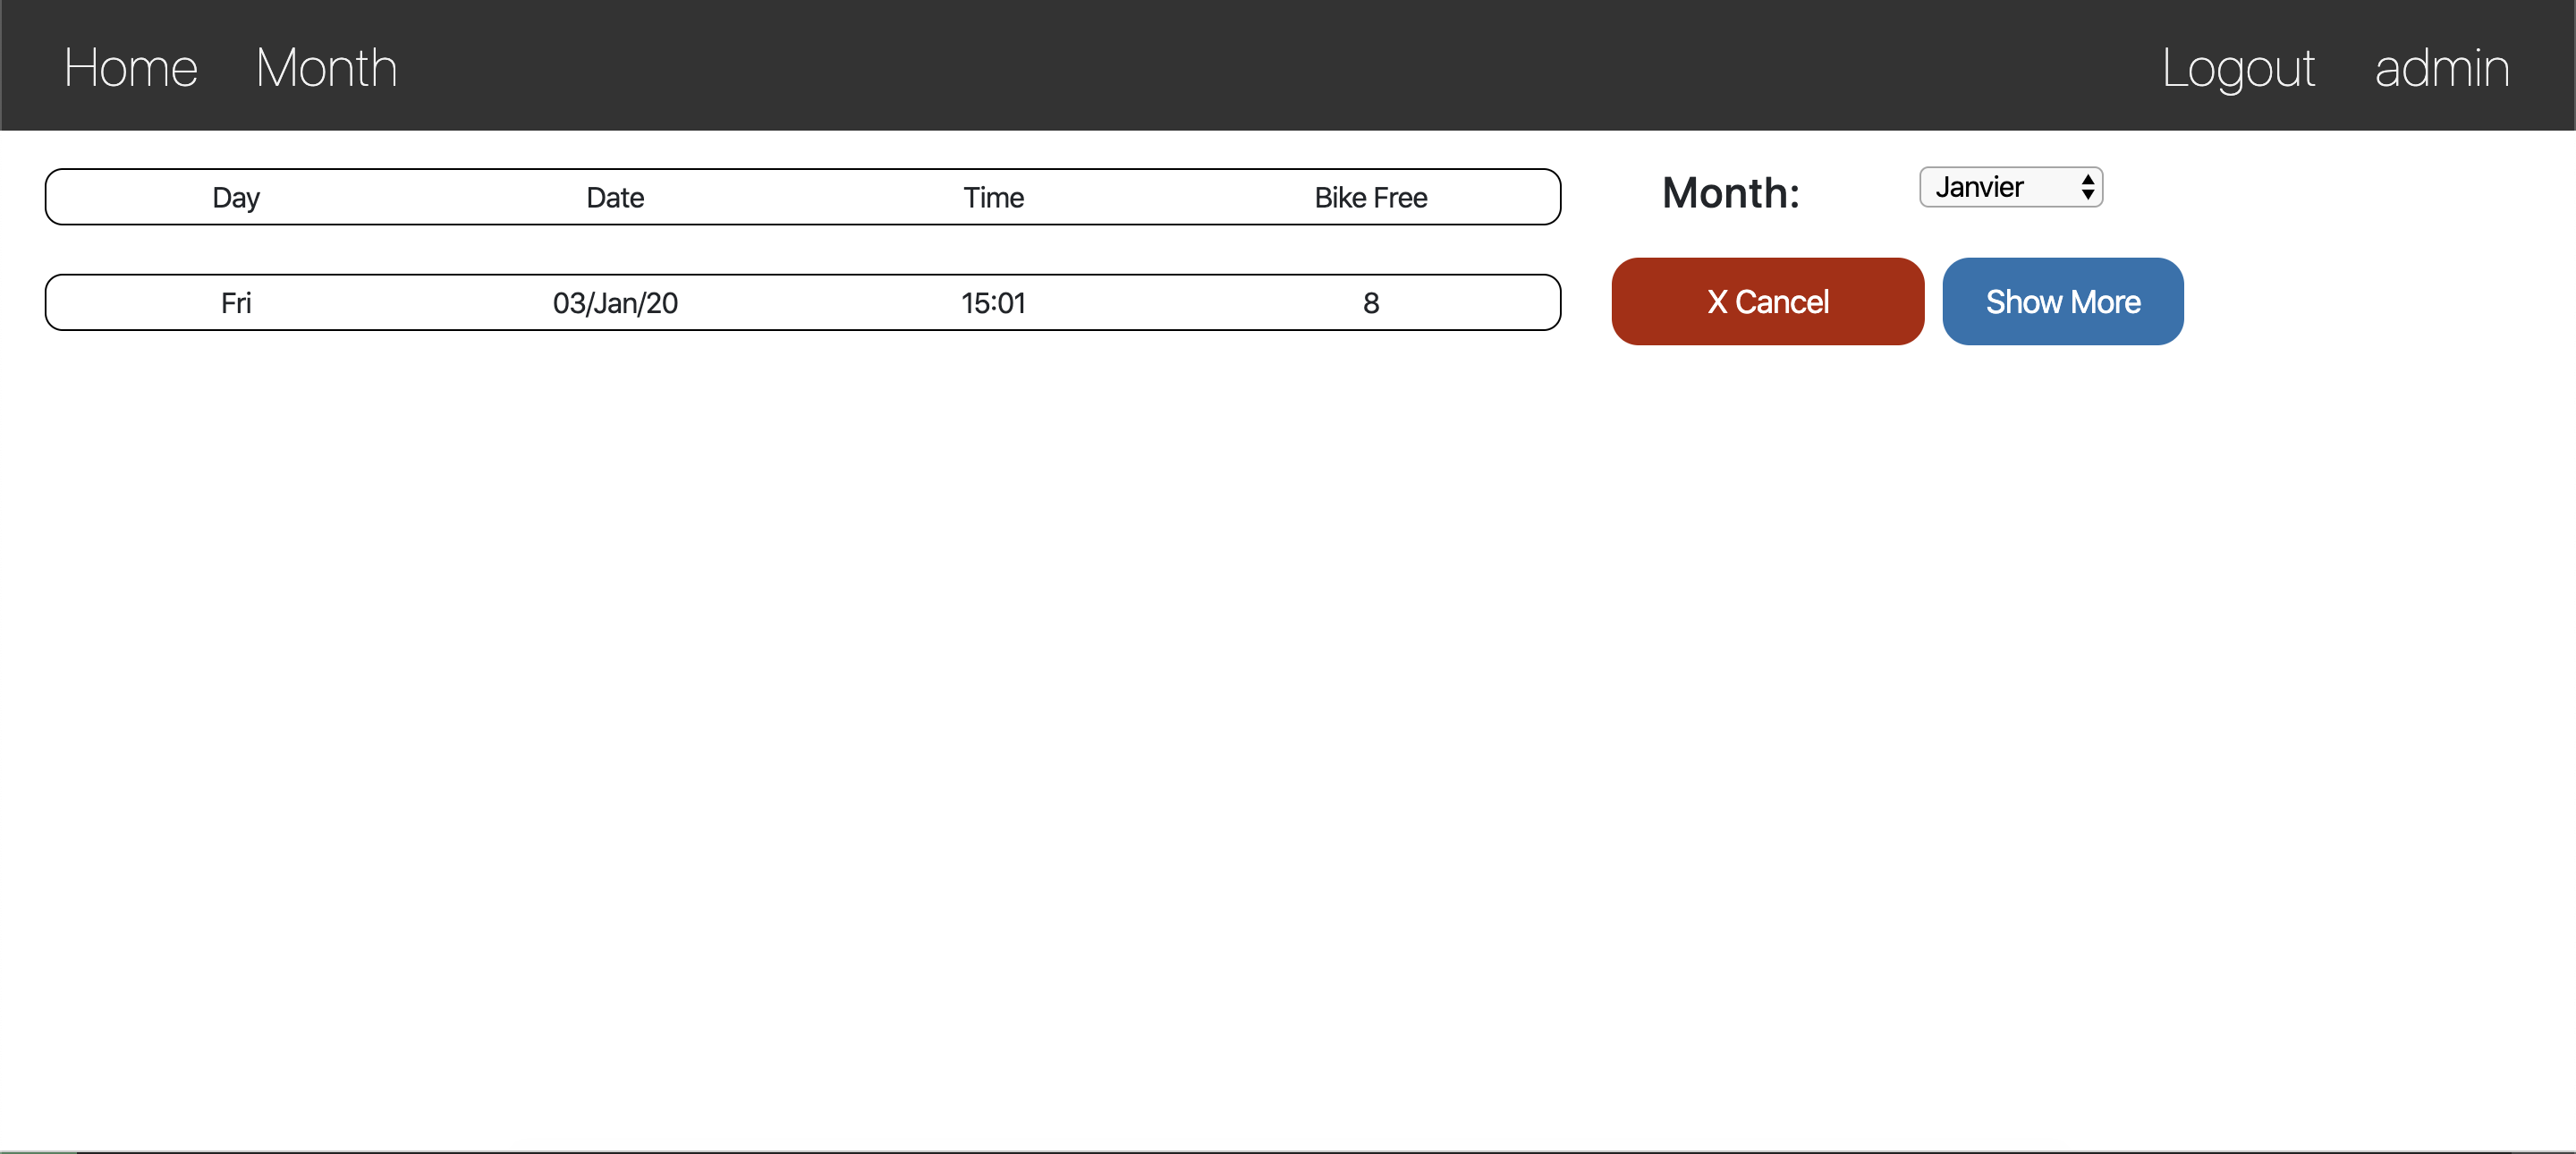
\includegraphics[width=0.8\linewidth, center]{Mockup/Admin-Session.png}
       	 	\caption{Page de gestion des sessions du mois pour l'administrateur}
       	\end{figure}
       	
	\newpage
	\subsection{Admin - Nouvelle session}
		\begin{figure}[h!]
       	 	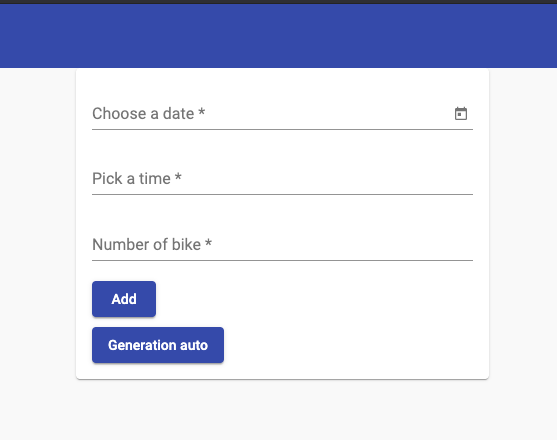
\includegraphics[width=0.8\linewidth, center]{Mockup/Admin-Nouvelle-Session.png}
       	 	\caption{Page de création d'une nouvelle session}
       	\end{figure}
       	
	\vspace{\baselineskip}
	\subsection{Admin - Abonnement}
		\begin{figure}[h!]
       	 	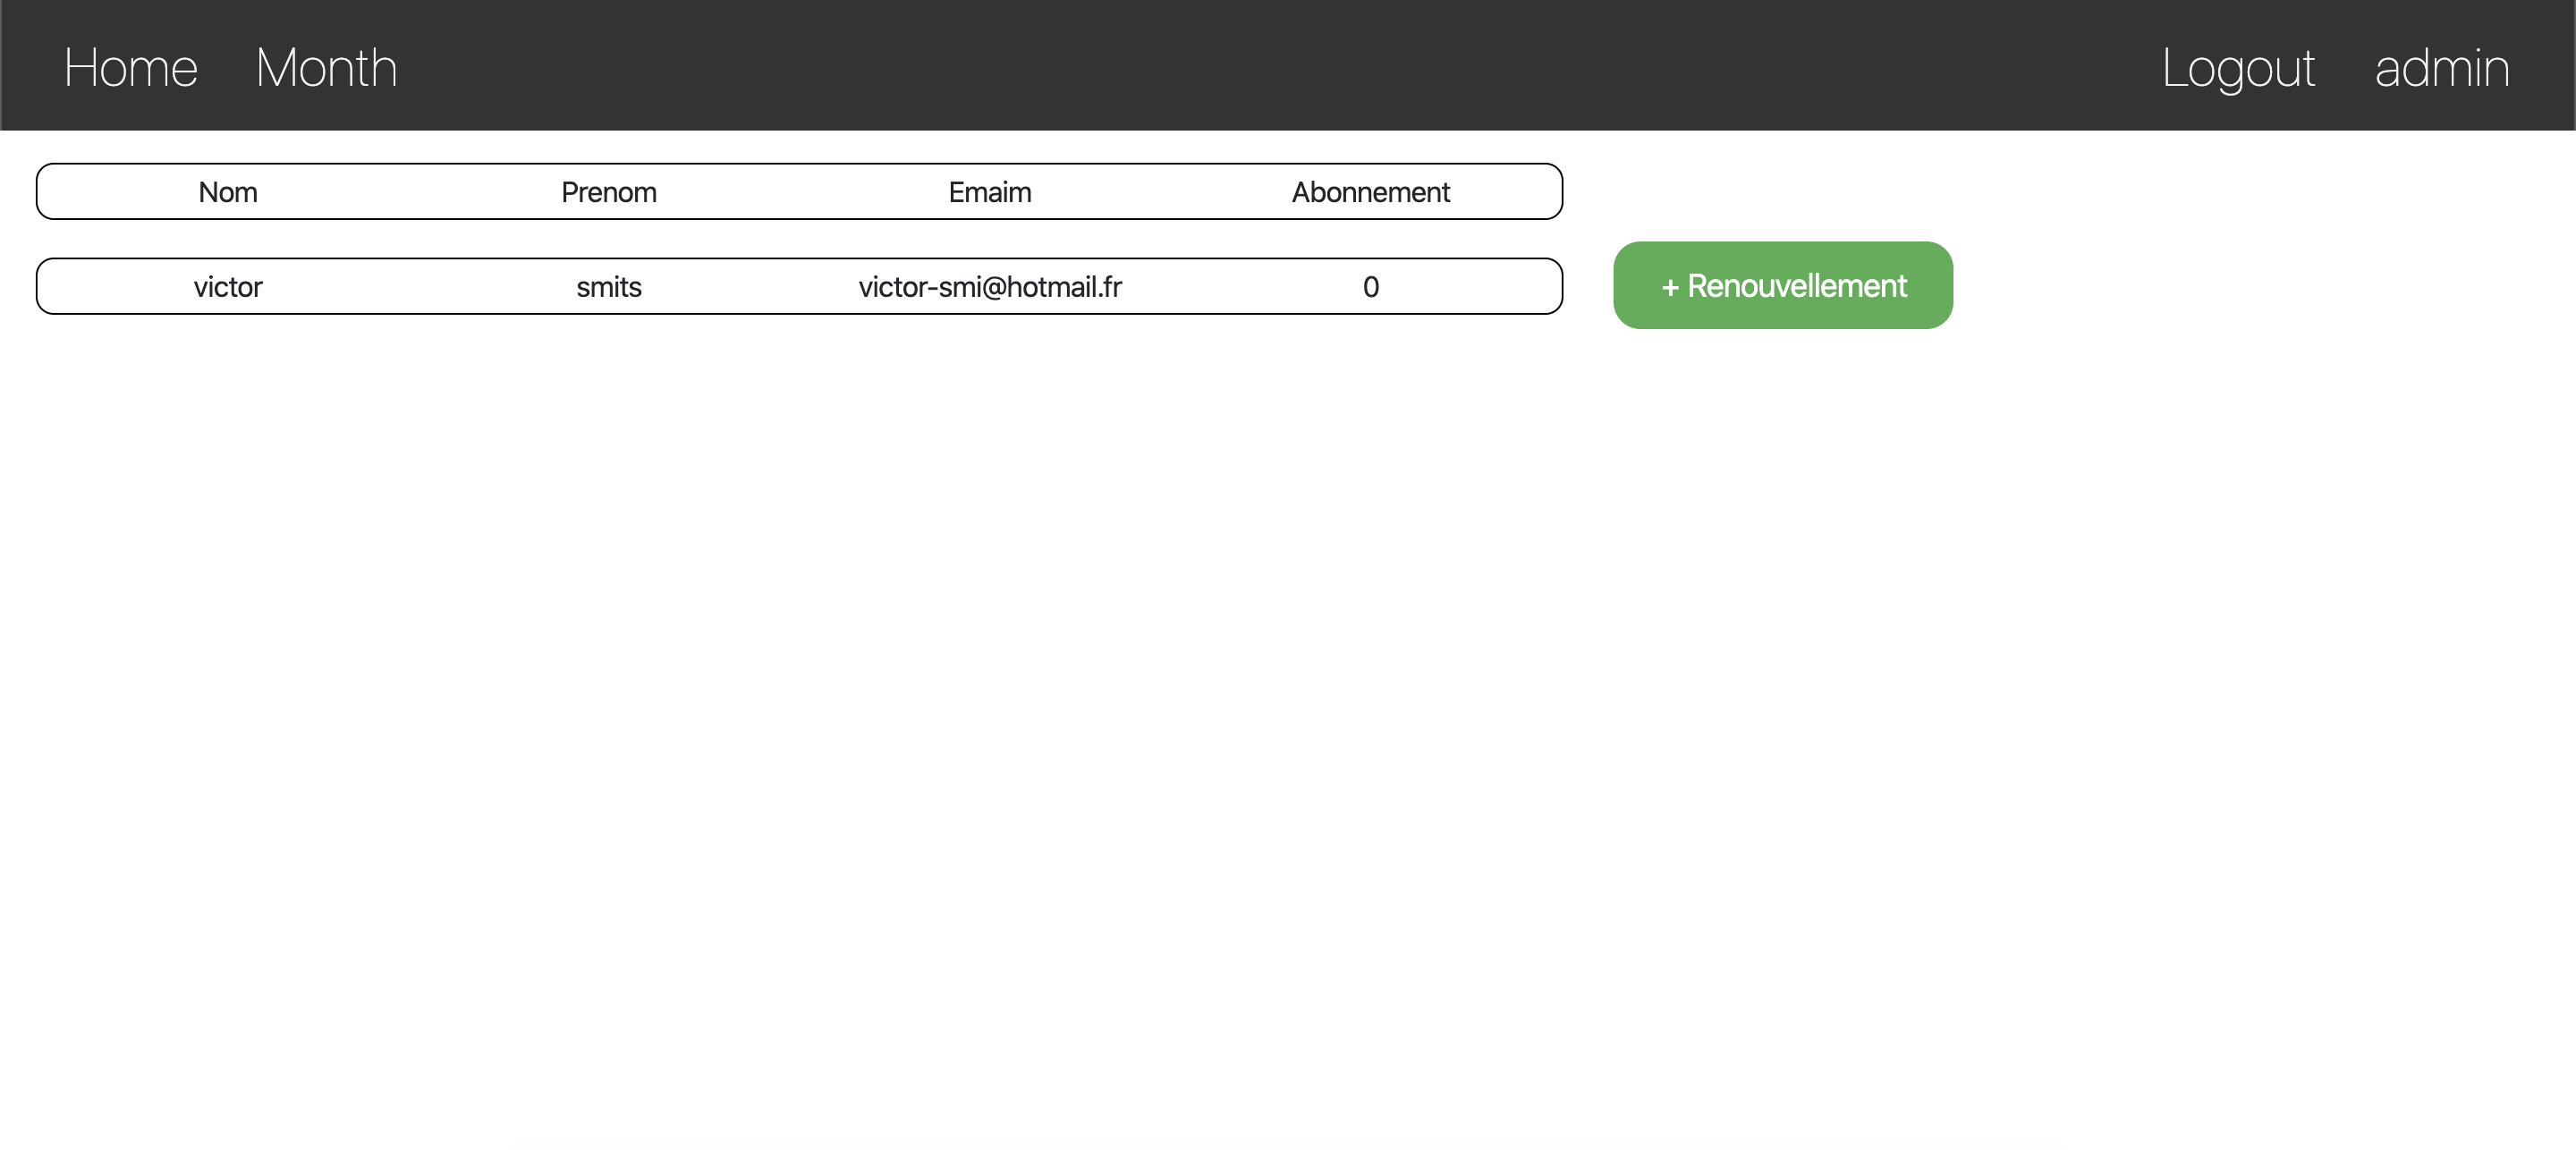
\includegraphics[width=0.8\linewidth, center]{Mockup/Admin-Abonnement.png}
       	 	\caption{Page de gestion des abonnements des utilisateurs}
       	\end{figure}
       	
	
	\newpage
	\subsection{Admin - Type Session}
		\begin{figure}[h!]
       	 	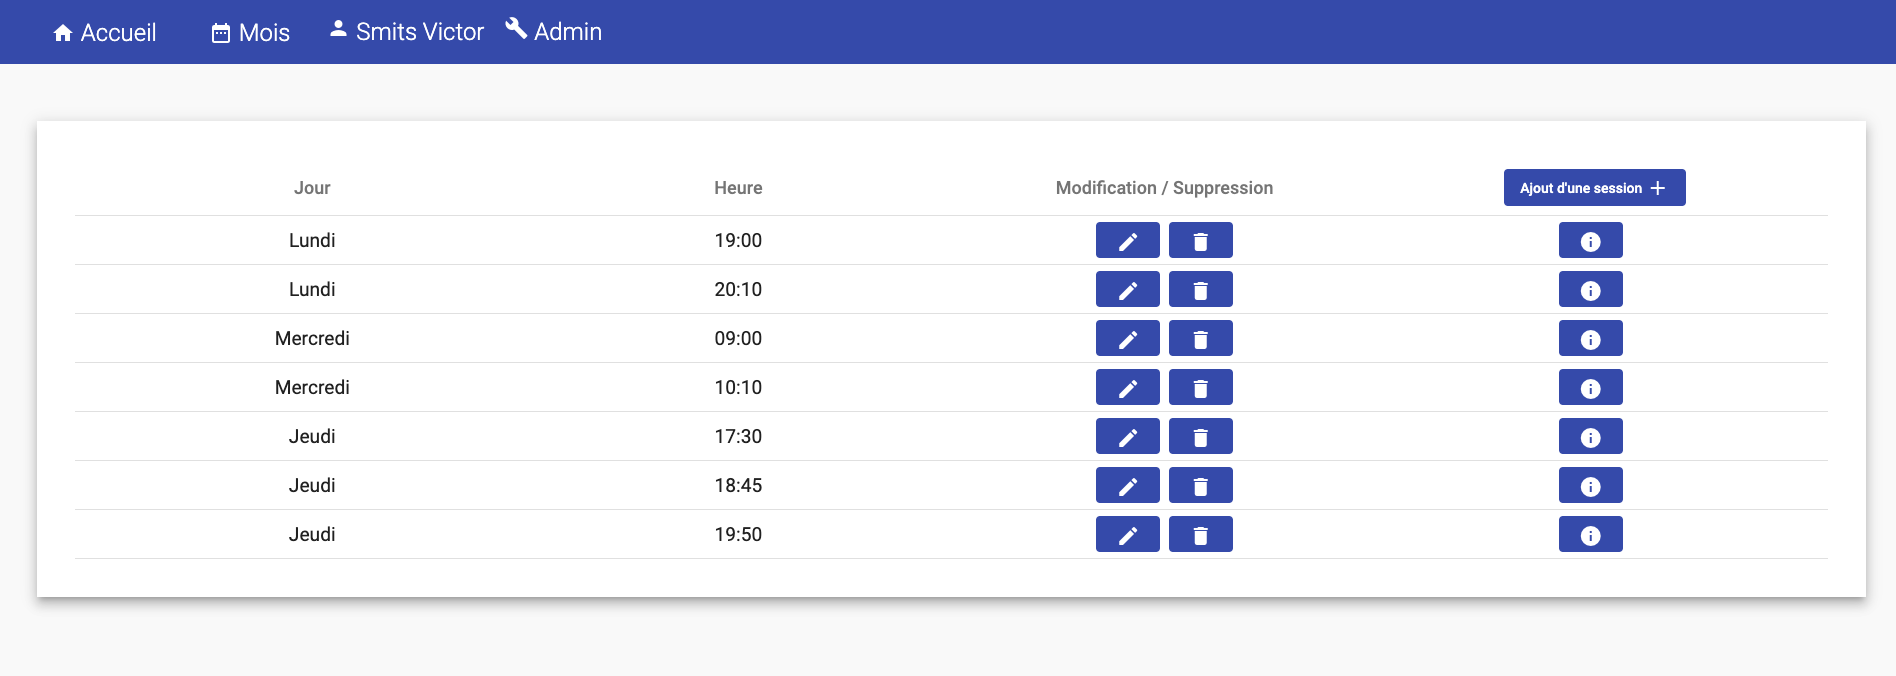
\includegraphics[width=0.8\linewidth, center]{Mockup/Admin-Type-Session.png}
       	 	\caption{Page de gestion des types de sessions}
       	\end{figure}



\chapter{Base de donnée}
\label{chap:Base de donnée}

	\vspace{\baselineskip}
	\section{Diagramme Entité relation}
	\begin{figure}[h!]
       	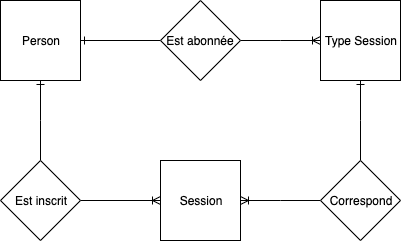
\includegraphics[width=0.8\linewidth, center]{Figures/Entite-relation.png}
       	\caption{Diagramme Relationnel}
	\end{figure}

\newpage
\section{Diagramme Relationnel}
	\begin{figure}[h!]
       	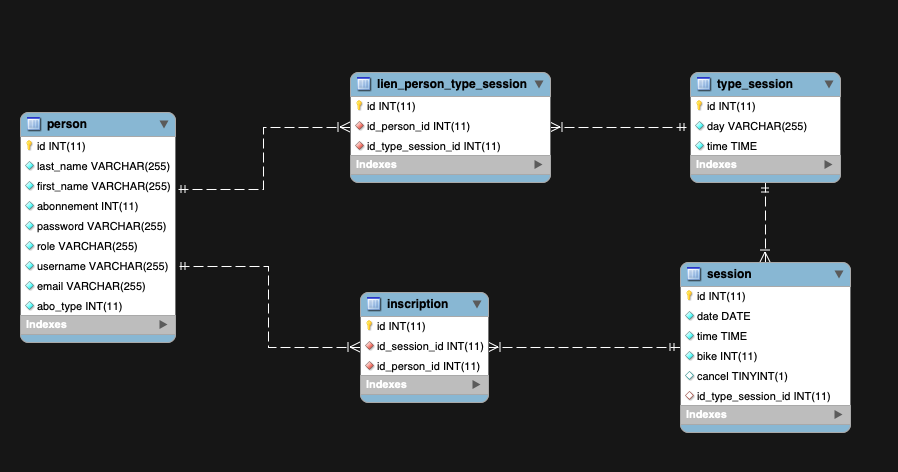
\includegraphics[width=\linewidth, center]{Figures/Diagramme-Relationnel}
       	 \caption{Diagramme Relationnel}
	\end{figure}
	
	
\section{Description des tables et des relations entre tables}
	\paragraph{}
		\begin{tabularx}{\linewidth}{|T{0.15\linewidth}|T{0.15\linewidth}|T{0.15\linewidth}|Y|}
			\hline
			Table & Table & Type & Description\\
			\hline	
			Person & Inscription & 1 à N & Une personne possède plusieurs inscriptions. \\
			\hline
			Session & Inscription & 1 à N & Une session à plusieurs inscriptions. \\
			\hline
			Session & Type Session & N à 1 & Plusieurs sessions corresponde à un type de sessions, un type de session peut correspondre à plusieurs sessions. \\
			\hline
			Person & Lien person type session & 1 à N & Une Personne possède plusieurs liens, plusieurs liens corresponde à une personne. \\
			\hline
			Type Session & Lien person type session & 1 à N & Un type de session possède plusieurs liens, plusieurs liens corresponde à un seul type de session. \\
			\hline
		\end{tabularx}
		
\vspace{\baselineskip}
\section{Description précise des champs}
	\subsection{Table : Person}
		\paragraph{}
			\begin{tabularx}{\linewidth}{|T{0.14\linewidth}|T{0.05\linewidth}|T{0.05\linewidth}|T{0.13\linewidth}|T{0.14\linewidth}|T{0.13\linewidth}|Y|}
				\hline
				Nom & Key & NN & Type & Référence & Intitulé & Commentaire \\
				\hline
				id & PK & O & int & & Identifiant & \\
				\hline
				last\_name & & O & varchar(45) & & Nom & \\
				\hline
				frist\_name & & O & varchar(45) & & Prenom & \\
				\hline
				abonnement & & O & int & & Nombre de session restante & \\
				\hline
				password & & O & varchar(45) & & Mot de passe crypté & \\
				\hline
				role & & O & varchar(45) & & Role sur le site & Default = role\_user \\
				\hline
				username & & O & varchar(45) & & Nom d'utilisateur & Unique \\
				\hline
				email & & O & varchar(45) & & Adresse Email & Unique \\
				\hline
				abo\_type & & O & int & & obonnement origine & \\
				\hline
			\end{tabularx}
	
	
	\subsection{Table : Session}
		\paragraph{}
			\begin{tabularx}{\linewidth}{|T{0.14\linewidth}|T{0.05\linewidth}|T{0.05\linewidth}|T{0.13\linewidth}|T{0.14\linewidth}|T{0.13\linewidth}|Y|}
				\hline
				Nom & Key & NN & Type & Référence & Intitulé & Commentaire \\
				\hline
				id & PK & O & int & & Identifiant & \\
				\hline
				date & & O & DATE & & date & \\
				\hline
				time & & O & Time & & heure & \\
				\hline
				bike & & O & int & & Nombre de vélo restante & \\
				\hline
				cancel & & O & Boolean & & Status de la session & Default = Null\\
				\hline
				id type session & FK & O & int & id / typeSession & Lien avec le type de session & Default = Null\\
				\hline
			\end{tabularx}
			
			
	\vspace{\baselineskip}
	\subsection{Table : Type\_Session}
		\paragraph{}
			\begin{tabularx}{\linewidth}{|T{0.14\linewidth}|T{0.05\linewidth}|T{0.05\linewidth}|T{0.13\linewidth}|T{0.14\linewidth}|T{0.13\linewidth}|Y|}
				\hline
				Nom & Key & NN & Type & Référence & Intitulé & Commentaire \\
				\hline
				id & PK & O & int & & Identifiant & \\
				\hline
				day & & O & varchar(45) & & code du jour & \\
				\hline
				time & & O & Time & & heure & \\
				\hline
			\end{tabularx}
			
			
	\vspace{\baselineskip}
	\subsection{Table : inscription}
		\paragraph{}
			\begin{tabularx}{\linewidth}{|T{0.14\linewidth}|T{0.05\linewidth}|T{0.05\linewidth}|T{0.13\linewidth}|T{0.14\linewidth}|T{0.13\linewidth}|Y|}
				\hline
				Nom & Key & NN & Type & Référence & Intitulé & Commentaire \\
				\hline
				id & PK & O & int & & Identifiant & \\
				\hline
				id\_session & FK & O & int & id / session & lien avec la session & \\
				\hline
				id\_person & FK & O & int & id / person & lien avec la person & \\
				\hline
			\end{tabularx}
			
			
	\vspace{\baselineskip}
	\subsection{Table : lien\_person\_type\_session}
		\paragraph{}
			\begin{tabularx}{\linewidth}{|T{0.2\linewidth}|T{0.05\linewidth}|T{0.05\linewidth}|T{0.06\linewidth}|T{0.15\linewidth}|T{0.13\linewidth}|Y|}
				\hline
				Nom & Key & NN & Type & Référence & Intitulé & Commentaire \\
				\hline
				id & PK & O & int & & Identifiant & \\
				\hline
				id\_type\_session & FK & O & int & id / type\_session & lien avec le type de session & \\
				\hline
				id\_person & FK & O & int & id / person & lien avec la person & \\
				\hline
			\end{tabularx}

\chapter{MVC}
\label{chap:MVC}

	\vspace{\baselineskip}
	\section{User Stories compatible Angular - Twig}
	\paragraph{}
		Seul l'aspect graphique changera entre la version Twig et la version Angular.
		Pour plus de détail rendez-vous au chapitre \ref{chap:Séparation backend frontend}
	
	\subsection{En tant qu’utilisateur, je dois pouvoir me connecter sur le site}
		\subsubsection{Différences}
	\begin{itemize}
		\item Réalisation d'une requête POST via l'api REST permettant d'effectuer l'authentification dans le backend. 
		\item Différences au niveau de l'aspect graphique de la page de connection. 
		\item Connection via l'adresse Email et non le nom d'utilisateur. 
		\item Redirection automatique de l'utilisateur vers la page de connection lors de l'accès au site si l'utilisateur n'est pas connecté.
		\item Utilisation d'un LoginAuthenticator afin de pouvoir authentifier l'utilisateur dans le backend. 
		\item Utilisation de coockies pour préserver les informations de l'utilisateur. 
	\end{itemize}

\newpage
\subsubsection{Diagramme de séquence}
	\begin{figure*}[h!]
		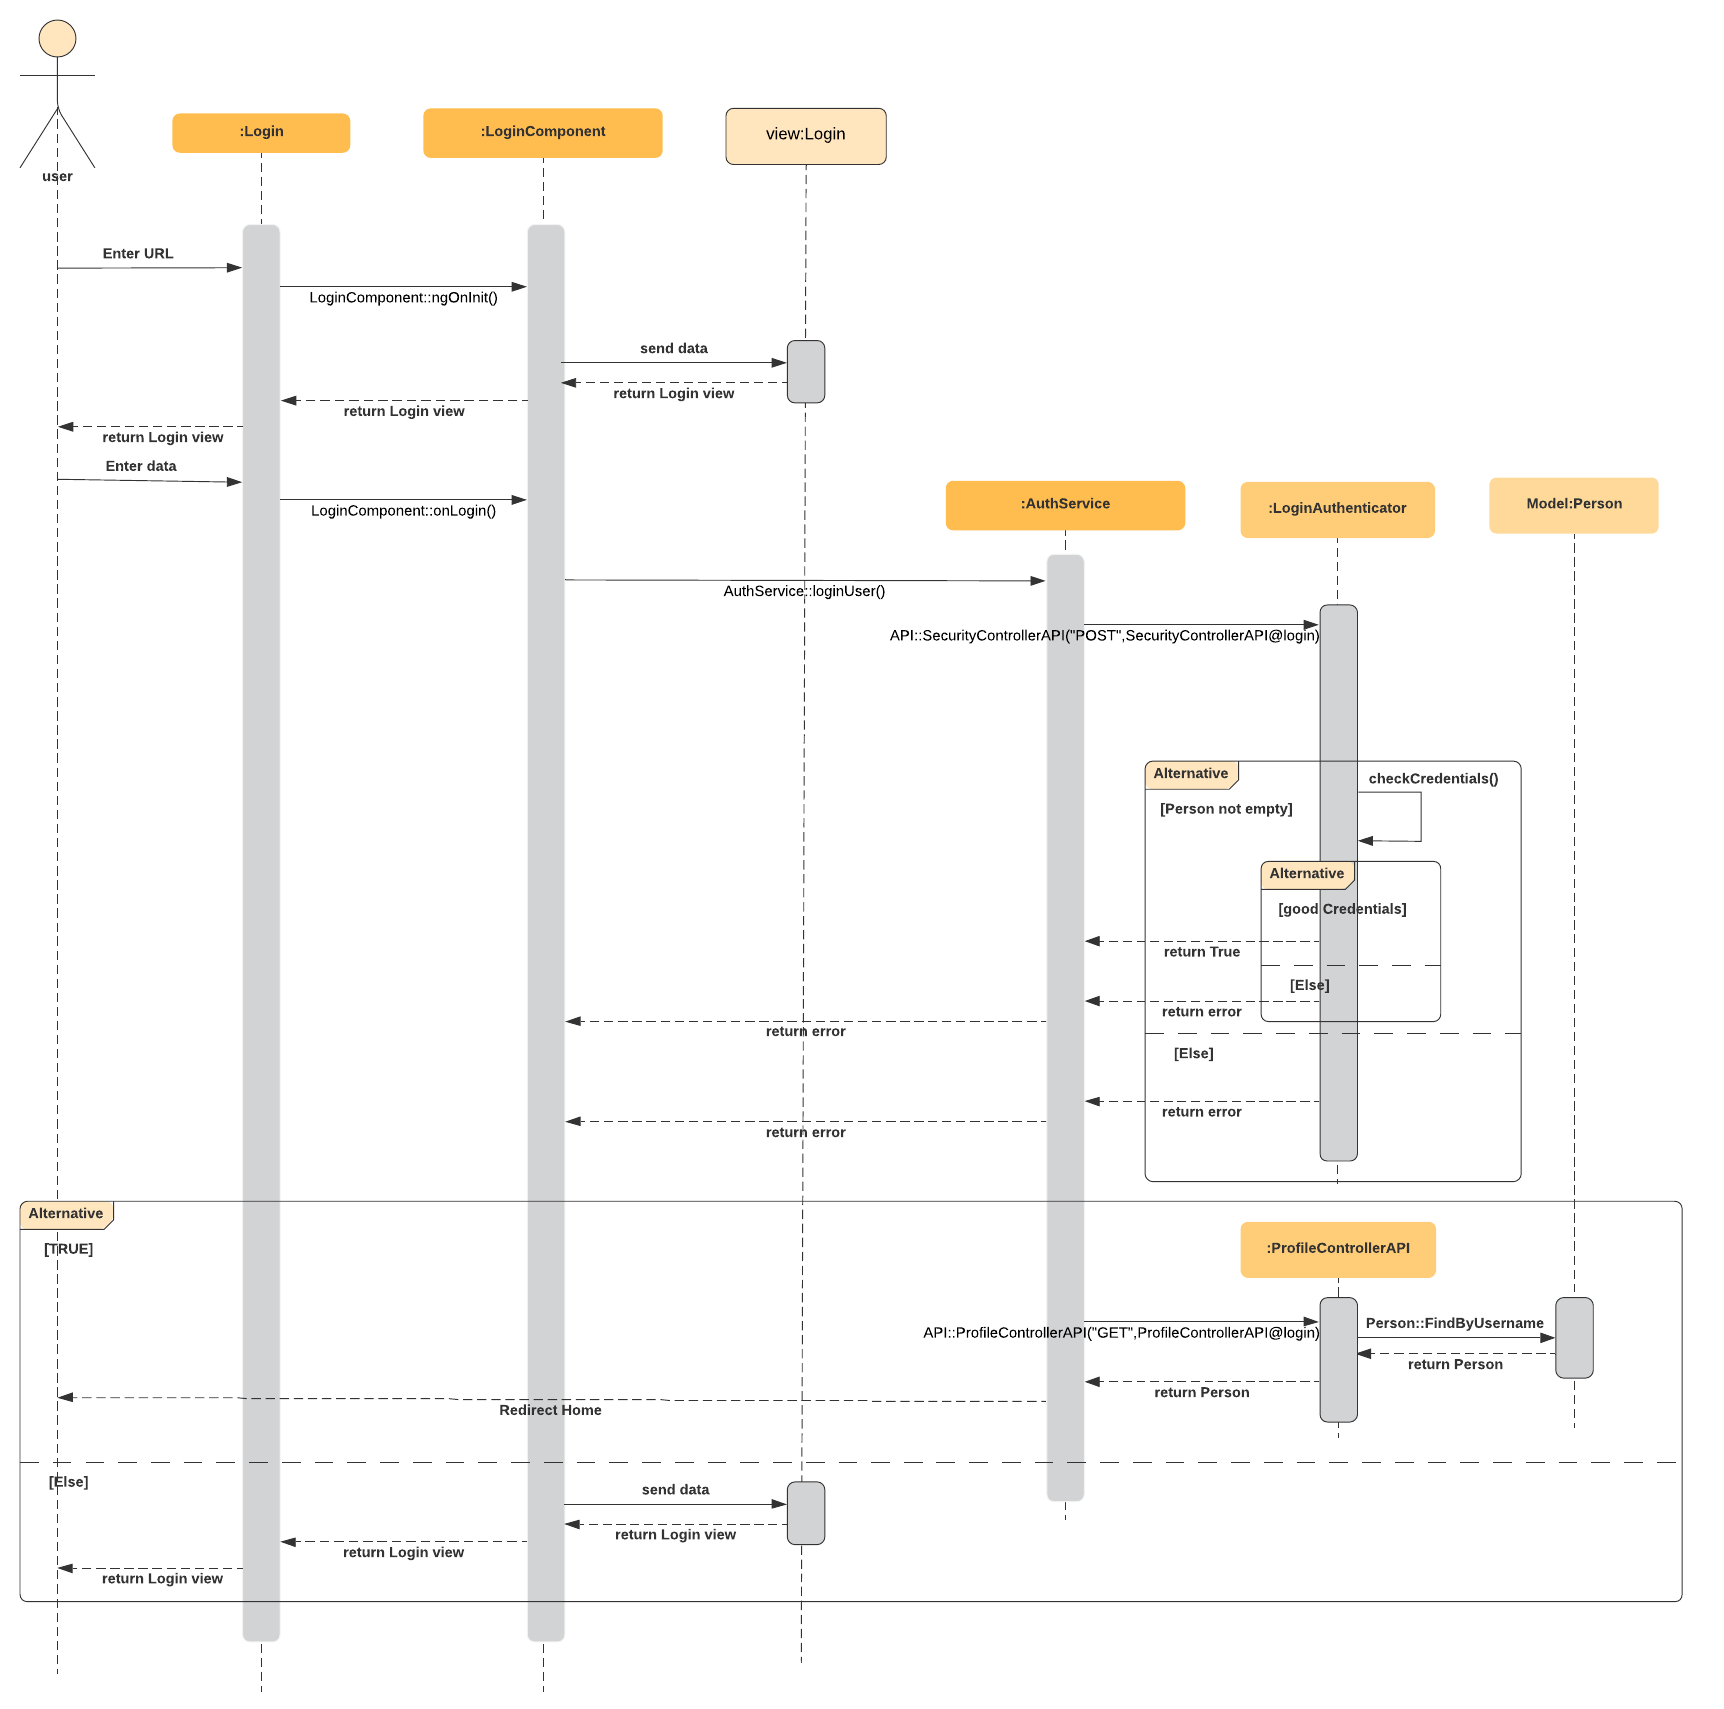
\includegraphics[width =\textwidth,center]{Diagramme/sequence-us0-angular}
		\caption{Diagramme de séquence de la connection d'un utilisateur}
	\end{figure*}

\newpage
\subsubsection{Scripts concernés}
	\begin{itemize}
		\item \Href{https://github.com/victorsmits/Aquabike/blob/master/frontend/src/app/service/api.service.ts}{api.service.ts}
		\item \Href{https://github.com/victorsmits/Aquabike/blob/master/frontend/src/app/service/auth.service.ts}{auth.service.ts}
		\item \Href{https://github.com/victorsmits/Aquabike/blob/master/backend/src/Controller/API/SecurityControllerAPI.php}{SecurityControllerAPI.php}
		\item \Href{https://github.com/victorsmits/Aquabike/blob/master/backend/src/Controller/API/ProfileControllerAPI.php}{ProfileControllerAPI.php}
		\item \Href{https://github.com/victorsmits/Aquabike/blob/master/frontend/src/app/login/login.component.ts}{login.component.ts}
		\item \Href{https://github.com/victorsmits/Aquabike/blob/master/frontend/src/app/login/login.component.html}{login.component.html}
		\item \Href{https://github.com/victorsmits/Aquabike/blob/master/backend/src/Entity/Person.php}{Person.php}
	\end{itemize}
	
	\vspace{\baselineskip}
	\subsection{En tant qu’utilisateur, je dois pouvoir me créer un compte sur le site}
		\begin{figure}[h]
	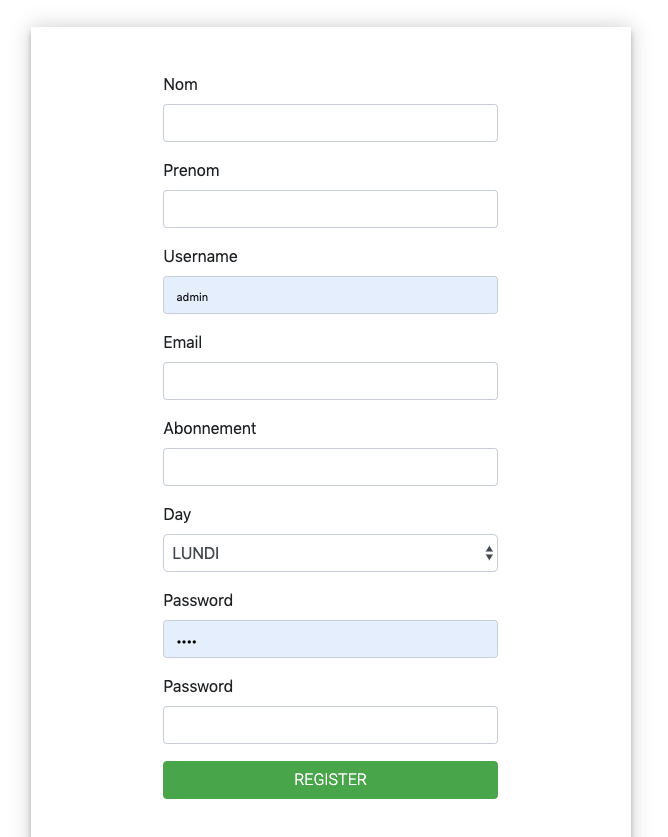
\includegraphics[width=0.5\textwidth,center]{Figures/us1-1}
	\caption{Formulaire d'inscription}
\end{figure}

\vspace{\baselineskip}
\begin{enumerate}
	\item L'utilisateur rentre ses information dans le formulaire. 
	\item L'utilisateur sélectionne le type de session à laquelle il est inscrit. 
	\item L'utilisateur clique sur \textit{Register} et attend la redirection. 
\end{enumerate}

\newpage
\subsubsection{Gestion des erreurs et sécurité}
	\paragraph{}
		\begin{itemize}
			\item L'utilisateur doit remplir tous les champs. Si un champ est manquant, une erreur apparaitra. 
			\item Le nom d'utilisateur et l'adresse Email sont uniques dans le système, s'il entre un Email ou nom d'utilisateur déjà existant, une erreur lui dira de corriger.
			\item L'utilisateur doit confirmer son mot de passe, si les mots de passe sont différents ou plus petits que 6 charactères il y aura un message d'erreur.
		\end{itemize}
		
\subsubsection{Diagramme de séquence}
	\begin{figure}[h]
		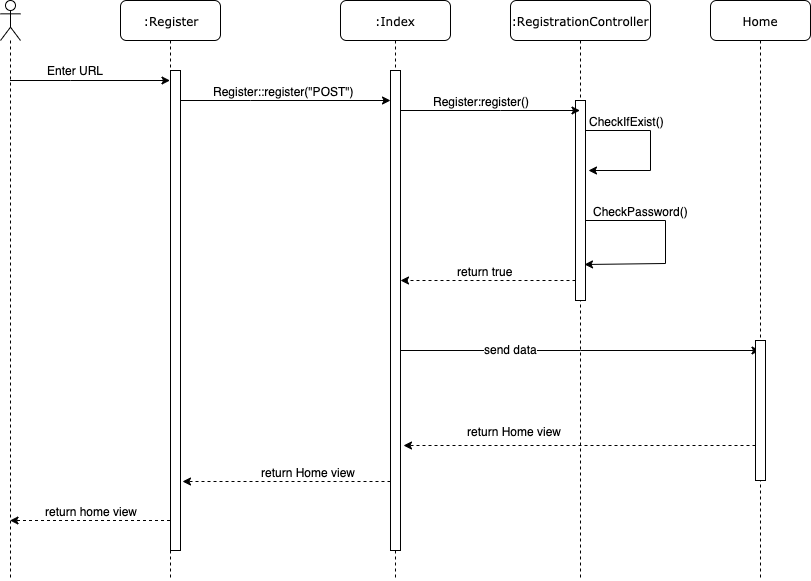
\includegraphics[width=0.8\textwidth,center]{Diagramme/sequence-us1}
		\caption{Diagramme de séquence de l'enregistrement d'un nouvelle utilisateur. }
	\end{figure}
	
	
\subsubsection{Scripts concernés}
	\begin{itemize}
		\item \Href{https://github.com/victorsmits/Aquabike/blob/master/backend/src/Controller/RegistrationController.php}{RegistrationController.php}
		\item \Href{https://github.com/victorsmits/Aquabike/blob/master/backend/templates/registration/register.html.twig}{register.html.twig}
		\item \Href{https://github.com/victorsmits/Aquabike/blob/master/backend/src/Entity/Person.php}{Person.php}
	\end{itemize}

	\vspace{\baselineskip}
	\subsection{En tant qu'utilisateur, je dois pouvoir sélectionner le mois et l'année pour afficher les sessions qui m'intéresse}
		\begin{figure*}[h]
	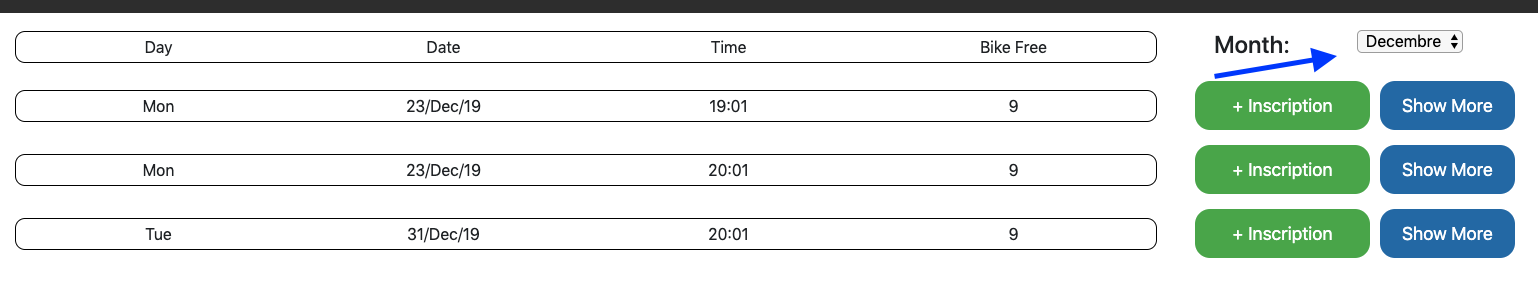
\includegraphics[width = 0.8\textwidth,center]{Figures/us2-1}
	\caption{selection du mois et de l'année}
\end{figure*}

\begin{enumerate}
	\item L'utilisateur choisit le mois et l'année. 
	\item la liste se rafraîchis afin de correspondre à la selection
\end{enumerate}
	
	\vspace{\baselineskip}
	\subsection{En tant qu’utilisateur, je dois pouvoir m’inscrire à une session un certain jour}
		\begin{figure*}[!h]
	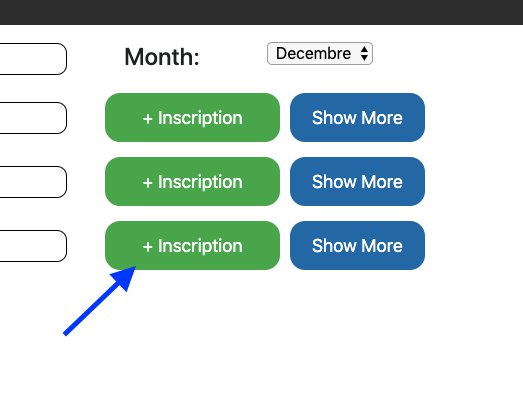
\includegraphics[width=0.5\textwidth,center]{Figures/us3-1}
	\caption{bouton d'inscritption}
\end{figure*}

\begin{enumerate}
	\item l'utilisateur choisit la session correspondant à sa demande.
	\item l'utilisateur clique sur le bouton  \textit{+ Inscription}
\end{enumerate}

\subsubsection{Gestion des erreurs}
	\begin{itemize}
		\item Si l'utilisateur ne possède plus d'abonnement, une erreur sera affichée lui signalant le problème. 
		\item Si la session est complète un message d'erreur sera affiché. 
	\end{itemize}
	
\subsubsection{Scripts concerné}
	\begin{itemize}
		\item \Href{https://github.com/victorsmits/Aquabike/blob/master/Symfony-Twig/src/Controller/MonthController.php}{MonthController.php}
		\item \Href{https://github.com/victorsmits/Aquabike/blob/master/Symfony-Twig/templates/month/month.html.twig}{month.html.twig}
		\item \Href{https://github.com/victorsmits/Aquabike/blob/master/Symfony-Twig/src/Entity/Session.php}{Session.php}
	\end{itemize}

	\vspace{\baselineskip}
	\subsection{En tant qu’utilisateur, je dois pouvoir être inscrit automatiquement à une session}
		\subsubsection{Différences}
	\begin{itemize}
		\item Réalisation de l'inscription automatique au session lors de l'enregistrement de l'utilisateurs. 
		\item Utilisation de type de session afin de facilité et de multiplier le choix des abonnements possible. 
		\item Possibilité pour un utilisateur de s'inscrire à plus de un type de session par semaine. 
		\item Sélection du type de session parmi une liste. 
	\end{itemize}

	\begin{figure*}[h!]
		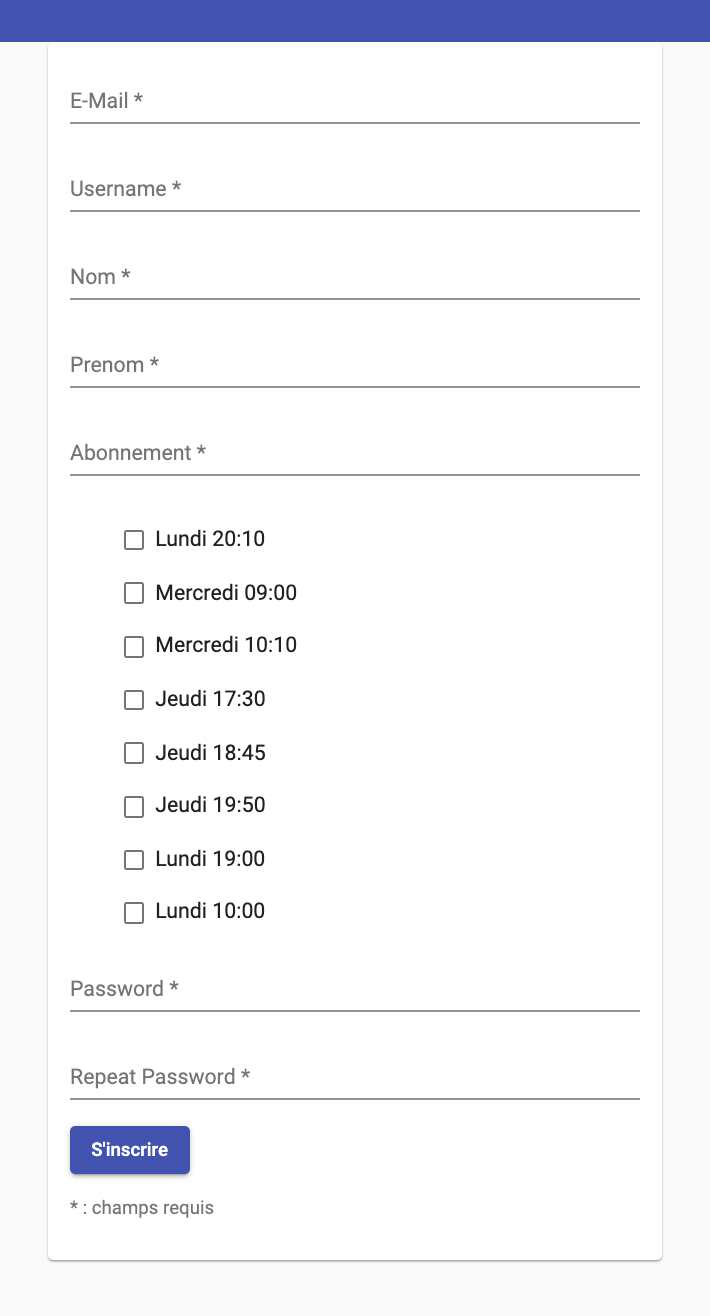
\includegraphics[width = 0.5\textwidth,center]{Figures/us4-1-angular}
		\caption{Formulaire d'inscription version angular}
	\end{figure*}
	
	
\newpage
\subsubsection{Diagramme de séquence}
	\begin{figure}[h]
		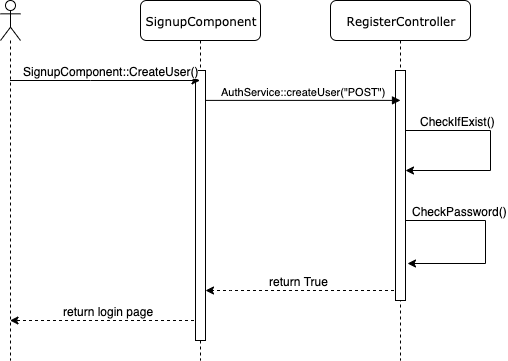
\includegraphics[width=\textwidth,center]{Diagramme/sequence-us1-angular}
		\caption{Diagramme de séquence de l'inscription automatique d'un utilisateur. }
	\end{figure}

\vspace{\baselineskip}
\subsubsection{Script concernés}
	\begin{itemize}
		\item \Href{https://github.com/victorsmits/Aquabike/blob/master/frontend/src/app/service/auth.service.ts}{auth.service.ts}
		\item \Href{https://github.com/victorsmits/Aquabike/blob/master/backend/src/Controller/API/SecurityControllerAPI.php}{SecurityControllerAPI.php}
		\item \Href{https://github.com/victorsmits/Aquabike/blob/master/backend/src/Entity/TypeSession.php}{TypeSession.php}
		\item \Href{https://github.com/victorsmits/Aquabike/blob/master/backend/src/Entity/Session.php}{Session.php}
		\item \Href{https://github.com/victorsmits/Aquabike/blob/master/backend/src/Entity/Inscription.php}{Inscription.php}
		\item \Href{https://github.com/victorsmits/Aquabike/blob/master/backend/src/Entity/Person.php}{Person.php}
		\item \Href{https://github.com/victorsmits/Aquabike/blob/master/frontend/src/app/signup/signup.component.ts}{signup.component.ts}
		\item \Href{https://github.com/victorsmits/Aquabike/blob/master/frontend/src/app/signup/signup.component.html}{signup.component.html}
	\end{itemize}
	
	\vspace{\baselineskip}
	\subsection{En tant qu’utilisateur, je dois pouvoir me désinscrire à une session}
		\begin{figure*}[h]
	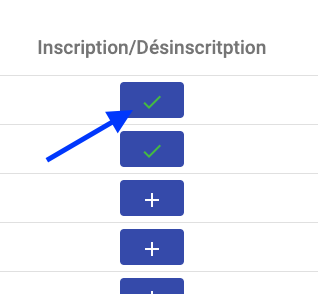
\includegraphics[width=0.5\textwidth,center]{Figures/us5-1}
	\caption{Bouton de désinscription à une session}
\end{figure*}

\begin{enumerate}
	\item L'utilisateur trouve la session qui l'interesse.
	\item Le check vert indique qu'il est inscrit.
	\item Il clique sur le bouton.
\end{enumerate}

\vspace{\baselineskip}
\subsubsection{Script concernés}
	\begin{itemize}
		\item \href{https://github.com/victorsmits/Aquabike/blob/master/backend/src/Controller/MonthController.php}{MonthController.php}
		\item \href{https://github.com/victorsmits/Aquabike/blob/master/backend/templates/registration/month.html.twig}{month.html.twig}
		\item \href{https://github.com/victorsmits/Aquabike/blob/master/backend/src/Entity/Person.php}{Person.php}
		\item \href{https://github.com/victorsmits/Aquabike/blob/master/backend/src/Entity/Inscription.php}{Inscription.php}
	\end{itemize}

	\vspace{\baselineskip}
	\subsection{En tant qu’utilisateur, je dois pouvoir voir qui est inscrit pour chaque session}
		\vspace{\baselineskip}
\begin{figure}[h]
	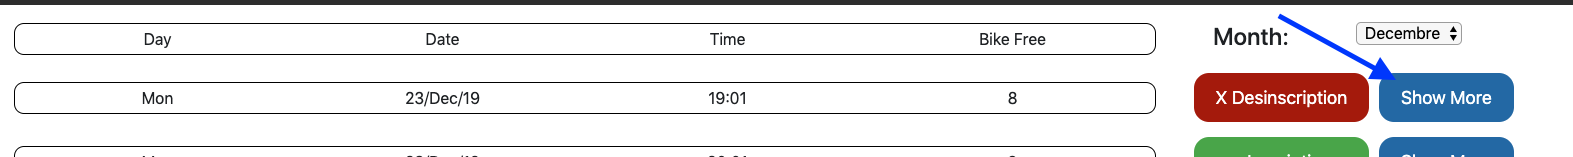
\includegraphics[width=0.9\textwidth,center]{Figures/us6-1}
	\caption{Bouton d'affichage}
\end{figure}

\begin{figure}[h]
	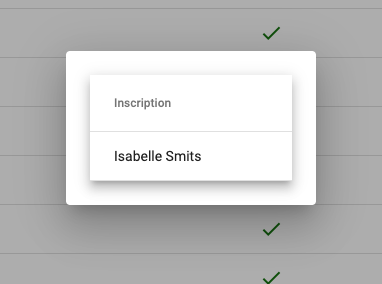
\includegraphics[width=0.5\textwidth,center]{Figures/us6-2}
	\caption{Liste Participant(e)s}
\end{figure}

\begin{enumerate}
	\item L'utilisateur trouve la session qui l'intéresse. 
	\item L'utilisateur clique sur le bouton information dans la colonne \textit{Liste Participant(e)s}. 
	\item Un tableau s'affiche avec la liste des inscrit(e)s. 
\end{enumerate}
	
	\newpage
	\subsection{En tant qu’utilisateur, je veux pouvoir voir dynamiquement le nombre de séance qui reste dans mon abonnement}
		\begin{enumerate}
	\item L'utilisateur clique sur son nom dans la bar de navigation.
	\item L'utilisateur est redirigé vers sa page de profil. 
	\item L'utilisateur retrouve l'information dans le cadre afficher sur la page.
\end{enumerate}

\vspace{\baselineskip}
\begin{figure}[h]
	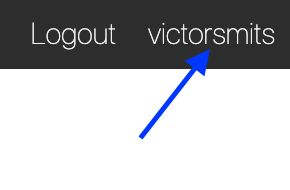
\includegraphics[width=0.5\textwidth,center]{Figures/us7-1}
	\caption{Bouton de navigation vers le profil}
\end{figure}

\vspace{\baselineskip}
\begin{figure}[h]
	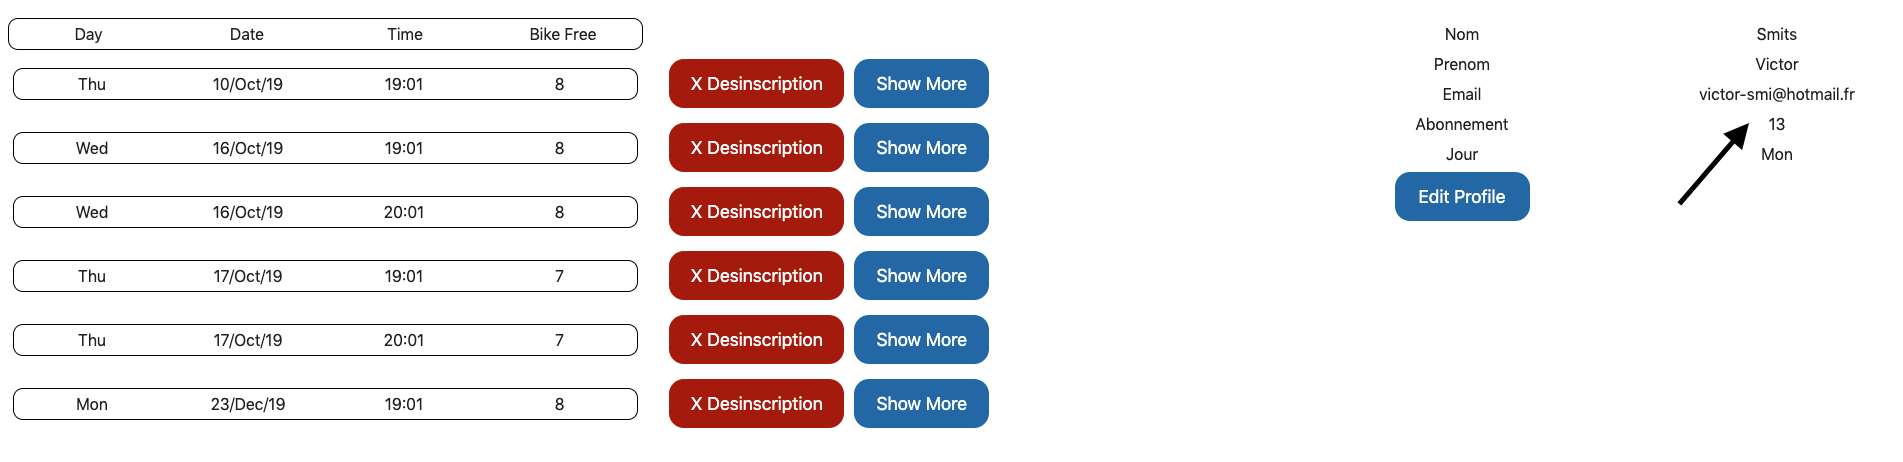
\includegraphics[width=0.9\textwidth,center]{Figures/us7-2}
	\caption{Nombre de séance restante dans l'abonnement}
\end{figure}


\vspace{\baselineskip}
\subsubsection{Script concernés}
	\begin{itemize}
		\item \Href{https://github.com/victorsmits/Aquabike/blob/master/backend/src/Controller/ProfileController.php}{ProfileController.php}
		\item \Href{https://github.com/victorsmits/Aquabike/blob/master/backend/templates/registration/profile.html.twig}{profile.html.twig}
		\item \Href{https://github.com/victorsmits/Aquabike/blob/master/backend/src/Entity/Person.php}{Person.php}
	\end{itemize}


	\vspace{\baselineskip}	
	\subsection{En tant qu'utilisateur, je veux pouvoir modifier mon profile}
		\begin{enumerate}
	\item L'utilisateur clique sur son nom dans la bar de navigation.
	\item L'utilisateur clique sur \textit{Profil} dans le menu déroulant.
	\item L'utilisateur clique sur le bouton edit au dessus de son profil. 
	\item Une fenêtre apparait. 
	\item L'utilisateur rentre les information qu'il souhaite changer. 
	\item L'utilisateur confirm en cliquant sur \textit{ok}
\end{enumerate}

\vspace{\baselineskip}
\begin{figure}[h]
	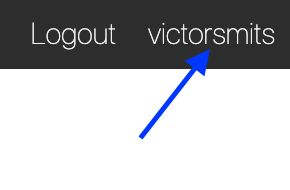
\includegraphics[width=0.4\textwidth,center]{Figures/us7-1}
	\caption{Bouton de navigation vers le profil}
\end{figure}

\begin{figure}[h]
	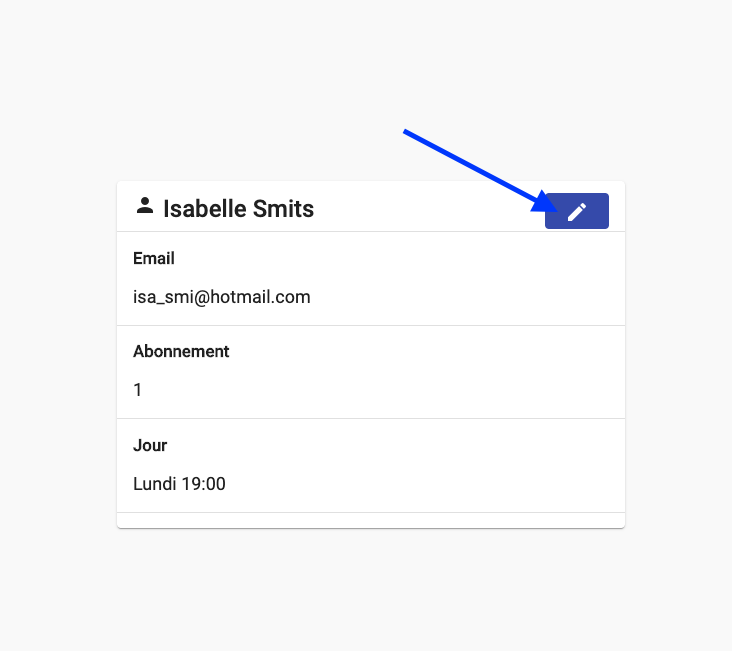
\includegraphics[width=0.4\textwidth,center]{Figures/us8-1}
	\caption{Bouton de modification du profil}
\end{figure}

\newpage
\begin{figure}[h]
	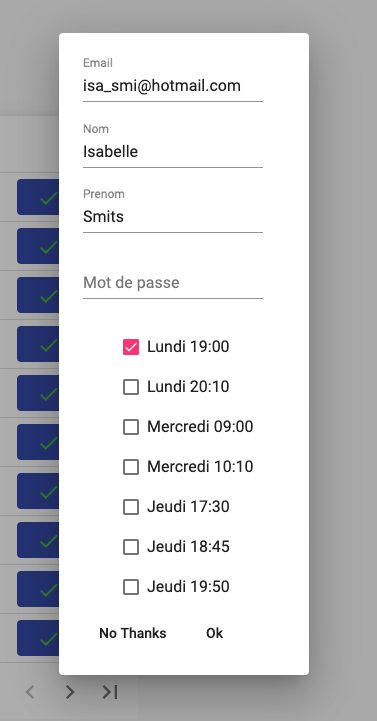
\includegraphics[width=0.4\textwidth,center]{Figures/us8-2}
	\caption{Fenêtre de modification des données du profil}
\end{figure}

	\vspace{\baselineskip}
	\subsection{En tant qu’administrateur, je dois pouvoir annuler une session}
		\subsubsection{Différences}
	\begin{itemize}
		\item Modification graphique du bouton d'annulation de la session. 
	\end{itemize}

\vspace{\baselineskip}
\subsubsection{Scripts concernés}
	\begin{itemize}
		\item \Href{https://github.com/victorsmits/Aquabike/blob/master/frontend/src/app/service/api.service.ts}{api.service.ts}
		\item \Href{https://github.com/victorsmits/Aquabike/blob/master/backend/src/Controller/API/SessionAdministrationControllerApi.php}{SessionAdministrationControllerApi.php}
		\item \Href{https://github.com/victorsmits/Aquabike/blob/master/backend/src/Entity/Session.php}{Session.php}
		\item \Href{https://github.com/victorsmits/Aquabike/blob/master/frontend/src/app/admin-session/admin-session.component.ts}{admin-session.component.ts}
		\item \Href{https://github.com/victorsmits/Aquabike/blob/master/frontend/src/app/admin-session/admin-session.component.html}{admin-session.component.html}
	\end{itemize}

	\newpage
	\subsection{En tant qu'administrateur, je dois pouvoir créer une nouvelle session peut importe la date}
		\subsubsection{Différence}
	\begin{itemize}
		\item Modification graphique du formulaire de création de session. 
	\end{itemize}
	
\vspace{\baselineskip}
\subsubsection{Script concernés}
	\begin{itemize}
		\item \href{https://github.com/victorsmits/Aquabike/blob/master/frontend/src/app/service/api.service.ts}{api.service.ts}
		\item \href{https://github.com/victorsmits/Aquabike/blob/master/backend/src/Controller/API/CreateSessionControllerApi.php}{CreateSessionControllerApi.php}
		\item \href{https://github.com/victorsmits/Aquabike/blob/master/backend/src/Entity/Session.php}{Session.php}
		\item \href{https://github.com/victorsmits/Aquabike/blob/master/frontend/src/app/admin-create-session/admin-create-session.component.ts}{admin-create-session.component.ts}
		\item \href{https://github.com/victorsmits/Aquabike/blob/master/frontend/src/app/admin-create-session/admin-create-session.component.html}{admin-create-session.component.html}
	\end{itemize}

	\newpage
	\subsection{En tant qu'administrateur, je dois pouvoir gérer les abonnement des utilisateurs}
		\subsubsection{Différence}
	\begin{itemize}
		\item Modification graphique de l'affichage des utilisateurs enregistré dans le système. 
	\end{itemize}

\vspace{\baselineskip}
\subsubsection{Script concernés}
	\begin{itemize}
		\item \href{https://github.com/victorsmits/Aquabike/blob/master/frontend/src/app/service/api.service.ts}{api.service.ts}
		\item \href{https://github.com/victorsmits/Aquabike/blob/master/backend/src/Controller/API/AbonnementControllerApi.php}{AbonnementControllerApi.php}
		\item \href{https://github.com/victorsmits/Aquabike/blob/master/backend/src/Entity/Person.php}{Person.php}
		\item \href{https://github.com/victorsmits/Aquabike/blob/master/frontend/src/app/admin-abo/admin-abo.component.ts}{admin-abo.component.ts}
		\item \href{https://github.com/victorsmits/Aquabike/blob/master/frontend/src/app/admin-abo/admin-abo.component.html}{admin-abo.component.html}
	\end{itemize}


\chapter{API}
\label{chap:API}


	\vspace{\baselineskip}
	\paragraph{}
	Renvoie un JSON contenant toute les sessions du jours ainsi que les insciptions.

\subsection{Requête}
	\subsubsection{paramètre du path}
		\paragraph{}
			Pas de Paramètre pour le path.
	
	\subsubsection{Content type}
		\paragraph{}
			text/plain
			
	\subsubsection{Body}
		\paragraph{}
			Pas de body pour la requête.

\subsection{Réponse}
	\subsubsection{Réussite}
		\paragraph{}
			Retourne code 200
			
	\subsubsection{Content-type}
		\paragraph{}
			application/json
	
	\subsubsection{Body}
		\begin{center}
			\begin{tabularx}{\textwidth}{| T{0.2122\textwidth} | S{0.22\textwidth} | S{0.15\textwidth} | S{0.3\textwidth} |}
				\hline
				Propriété & Type & Obligatoire & Description \\
				\hline
				id & int & O & Id de la session. \\
				\hline
				Date & DateTime & O & Date de la session. \\
				\hline
				Time & DateTime & O & Heure de la session. \\
				\hline
				Bike & int & O & Nombre de vélo disponible pour la session. \\
				\hline
				Cancel & Boolean & O & Etats de la session. \\
				\hline
				IdTypeSession & int & O & id du type de session correspondant. \\
				\hline
				idInscription & List & O & Liste des participants. \\
				\hline
				idPerson & Person & O & Identité du participant. \\
				\hline
				lastName & String & O & Nom du participant. \\
				\hline
				firstName & String & O & Prénom du participant. \\
				\hline
			\end{tabularx}
		\end{center}
		
		\newpage
		\paragraph{Exemple JSON}
			\paragraph{}
			\begin{lstlisting}[language=json,firstnumber=1]
{
  id: 15,
  Date: "2019/12/23 00:00",
  time: "1970/01/01 19:00",
  bike: 8,
  Cancel: false,
  IdTypeSession: 1,
  idInscription: [{
  	0: {
  	  id: 45,
		idSession: 15,
		  idPerson: {
			  id: 49,
			  lastName: "Isabelle",
			  firstName: "Smits"
			}
		},
	}]
}
\end{lstlisting}
			
			
	\subsubsection{Code}
		\paragraph{}
			\Href{https://github.com/victorsmits/Aquabike/blob/master/backend/src/Controller/API/HomeControllerApi.php}{HomeControllerApi.php}


\chapter{Séparation backend frontend}
\label{chap:Séparation backend frontend}

	\vspace{\baselineskip}
	\paragraph{}
	Pour la séparation backend-frontend nous avons utiliser l'api REST qui nous permet de séparer les action sur la base de donnée et l'interface de l'application web tout en permettant la transmission des donnée grâce au format JSON.
	L'ensemble des requête réaliser si dessous ainsi que leur explication est expliqué dans le chapitre \ref{chap:API}. 
	
\paragraph{}
	La majorité des User Stories sont comparable et applicable au 2 architectures, cependant certaine de c'est User Stories ne sont implémenté qu'uniquement dans la partie Angular. C'est User Stories sont expliqués et illustrer ci-dessous. 

\newpage
\section{User Stories compatible Angular uniquement}
	\paragraph{}
		C'est User Stories on été ajouter part après la création du twig, soit pour faciliter l'exécution d'élément, soit dans le but d'ajouter de nouvelle fonctionnalité. 
	
	\subsection{En tant qu'administrateur, je dois pouvoir créer un type de session}
		\begin{enumerate}
	\item L'administrateur se connecte au site avec ses identifiant. 
	\item Un nouveau bouton de navigation apparait dans la bar de navigation. 
	\item L'administrateur clique sur le bouton \textit{Admin}
	\item Il sélectionne \textit{Type Session} dans le menu déroulant. 
	\item L'administrateur atterris sur la page de gestion des type de sessions. 
	\item Il clique sur \textit{Ajout d'une session +}
	\item Un formulaire apparait et il le remplis avec les bonne information (jour - heure [hh:mm])
	\item Il clique sur \textit{ok} 
\end{enumerate}

\vspace{\baselineskip}
\begin{figure}[h]
	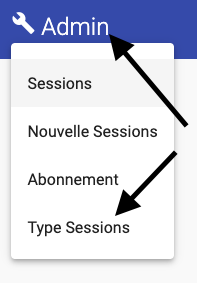
\includegraphics[width=0.3\textwidth,center]{Figures/us12-1}
	\caption{Bouton de navigation de l'administrateur}
\end{figure}

\newpage
\begin{figure}[h]
	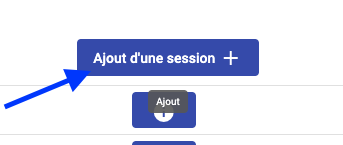
\includegraphics[width=0.5\textwidth,center]{Figures/us12-2}
	\caption{Bouton d'ajout d'un type de session}
\end{figure}

\vspace{\baselineskip}
\begin{figure}[h]
	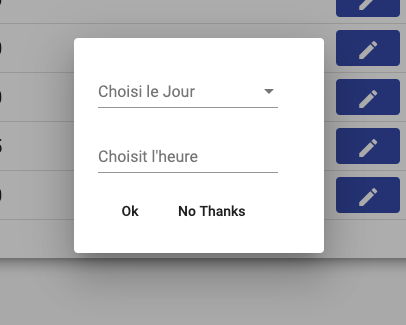
\includegraphics[width=0.5\textwidth,center]{Figures/us12-3}
	\caption{Page d'ajout du type de session}
\end{figure}

\vspace{\baselineskip}
\subsubsection{Gestion des erreurs}
	\begin{itemize}
		\item 2 types de sessions identiques ne peuvent exister, lors de la creation d'un type de session, une vérification se fait et, si le type de session existe deja, une erreur apparait.
		\item Si une erreur apparait durant la création du type de session, elle s'affichera au-dessus du formulaire. 
	\end{itemize}

\newpage
\subsubsection{Diagramme de séquence}
	\begin{figure}[h]
		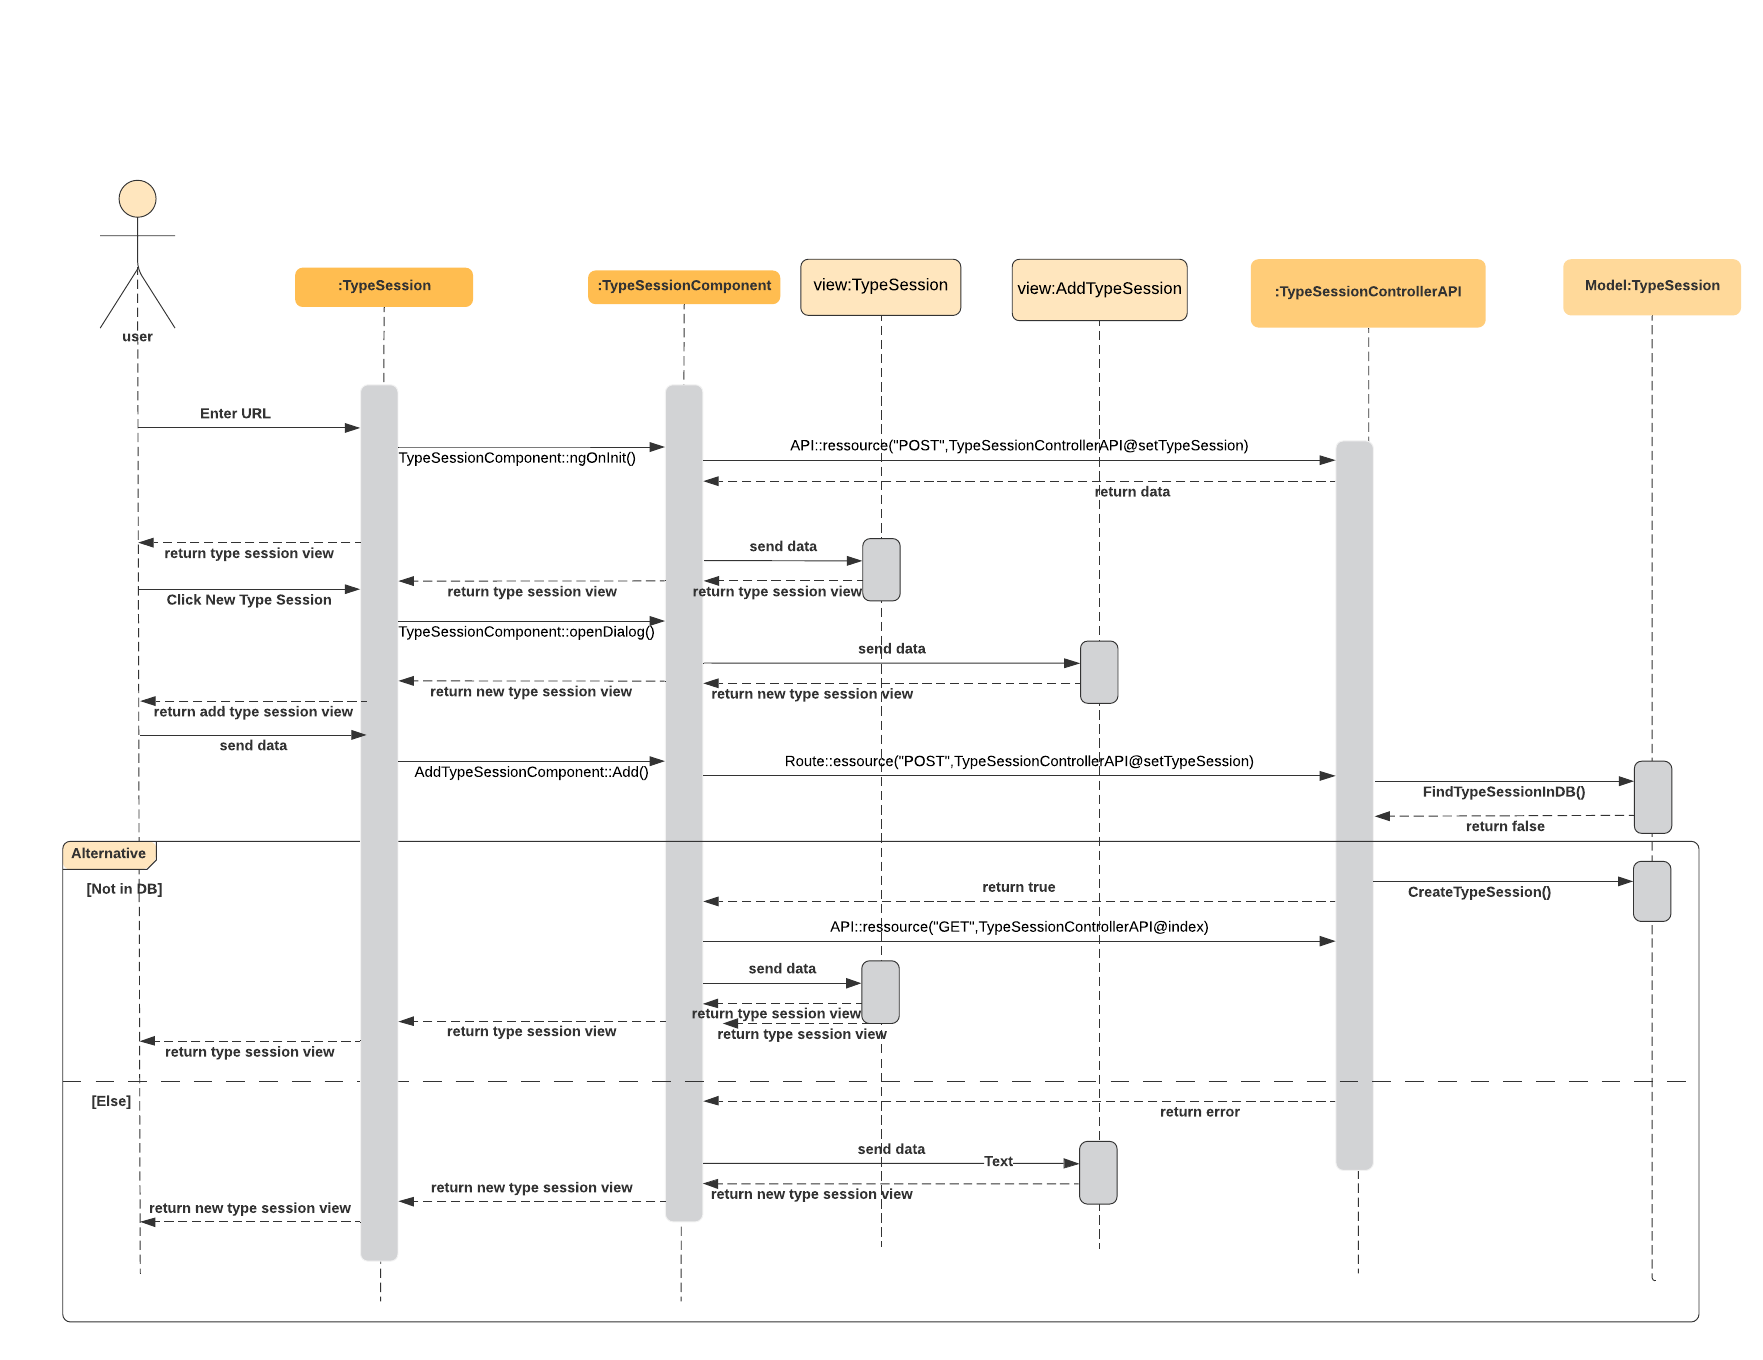
\includegraphics[width=\textwidth,center]{Diagramme/sequence-us12}
		\caption{Diagramme de séquence de l'ajout d'un type de session}
	\end{figure}

\subsubsection{Script concerné}
	\begin{itemize}
		\item \Href{https://github.com/victorsmits/Aquabike/blob/master/backend/src/Controller/API/RegistrationControllerApi.php}{RegistrationControllerApi.php}
		\item \Href{https://github.com/victorsmits/Aquabike/blob/master/backend/src/Entity/TypeSession.php}{TypeSession.php}
		\item \Href{https://github.com/victorsmits/Aquabike/blob/master/frontend/src/app/type-session/add-type-session.component.ts}{add-type-session.component.ts}
		\item \Href{https://github.com/victorsmits/Aquabike/blob/master/frontend/src/app/type-session/add-type-session.component.html}{add-type-session.component.html}
	\end{itemize}

	
	\newpage
	\subsection{En tant qu'administrateur, je veux pouvoir modifier un type de session}
		\begin{enumerate}
	\item L'administrateur se connecte au site avec ses identifiant. 
	\item Un nouveau bouton de navigation apparait dans la bar de navigation. 
	\item L'administrateur clique sur le bouton \textit{Admin}
	\item Il sélectionne \textit{Type Session} dans le menu déroulant. 
	\item L'administrateur atterris sur la page de gestion des type de sessions. 
	\item Il clique sur le bouton edit
	\item Un formulaire apparait et il le remplis avec les bonne information (jour - heure [hh:mm])
	\item Il clique sur \textit{ok} 
\end{enumerate}

\vspace{\baselineskip}
\begin{figure}[h]
	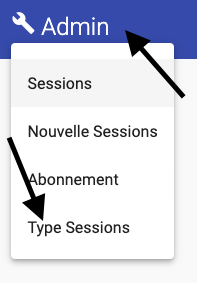
\includegraphics[width=0.4\textwidth,center]{Figures/us13-1}
	\caption{Menu de l'administrateur}
\end{figure}

\newpage
\begin{figure}[h]
	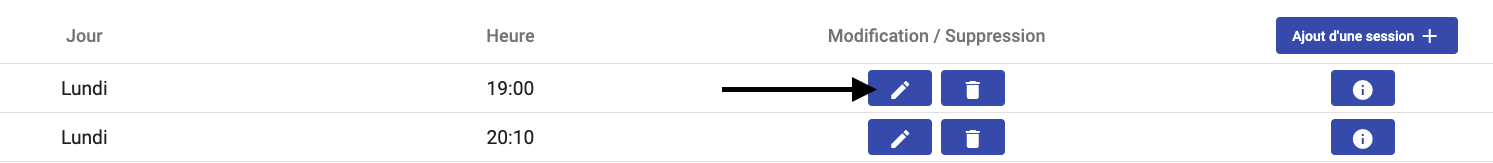
\includegraphics[width=0.9\textwidth,center]{Figures/us13-2}
	\caption{Bouton de modification du type de session}
\end{figure}

\vspace{\baselineskip}
\begin{figure}[h]
	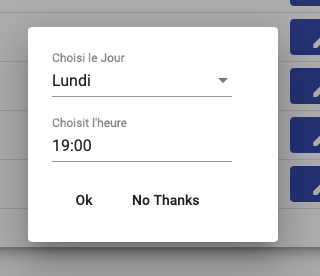
\includegraphics[width=0.4\textwidth,center]{Figures/us13-3}
	\caption{Formulaire de modification du type de session}
\end{figure}

\subsubsection{Gestion des erreurs}
	\paragraph{}
		Chaque type de sessions est unique, si l'administrateur rentre des informations correspondant à un type de sessions deja existant, une erreur apparaitra au dessus du formulaire.
	
	\newpage
	\subsection{En tant qu'administrateur, je veux pouvoir supprimer un type de session}
		\begin{enumerate}
	\item L'administrateur se connecte au site avec ses identifiant. 
	\item Un nouveau bouton de navigation apparait dans la bar de navigation. 
	\item L'administrateur clique sur le bouton \textit{Admin}
	\item Il sélectionne \textit{Type Session} dans le menu déroulant. 
	\item L'administrateur atterris sur la page de gestion des type de sessions. 
	\item Il clique sur le bouton supprimer
	\item Une fenêtre de confirmation apparait. 
	\item Il clique sur \textit{OUI!} 
\end{enumerate}


\begin{figure}[h]
	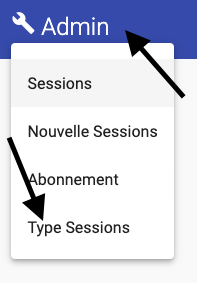
\includegraphics[width=0.4\textwidth,center]{Figures/us13-1}
	\caption{Menu de l'administrateur}
\end{figure}

\vspace{\baselineskip}
\begin{figure}[h]
	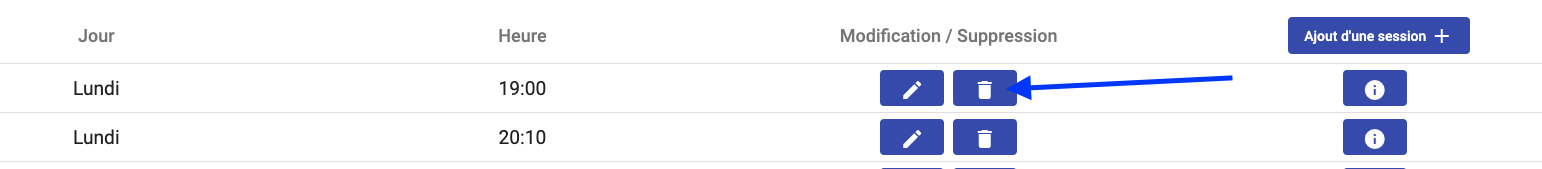
\includegraphics[width=0.9\textwidth,center]{Figures/us14-1}
	\caption{Bouton de suppression du type de session}
\end{figure}

\newpage
\begin{figure}[h]
	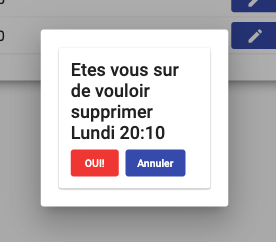
\includegraphics[width=0.4\textwidth,center]{Figures/us14-2}
	\caption{Fenêtre de confirmation de suppression}
\end{figure}

\subsubsection{Script concerné}
	\begin{itemize}
		\item \href{https://github.com/victorsmits/Aquabike/blob/master/backend/src/Controller/API/RegistrationControllerApi.php}{RegistrationControllerApi.php}
		\item \href{https://github.com/victorsmits/Aquabike/blob/master/backend/src/Entity/TypeSession.php}{TypeSession.php}
		\item \href{https://github.com/victorsmits/Aquabike/blob/master/frontend/src/app/type-session/del-type-session.component.ts}{del-type-session.component.ts}
		\item \href{https://github.com/victorsmits/Aquabike/blob/master/frontend/src/app/type-session/del-type-session.component.html}{del-type-session.component.html}
	\end{itemize}

	
	\vspace{\baselineskip}
	\vspace{\baselineskip}
	\subsection{En tant qu'administrateur, je veux pouvoir supprimer un utilisateur du système}
		\begin{enumerate}
	\item L'administrateur se connecte au site avec ses identifiants. 
	\item Un nouveau bouton de navigation apparait dans la barre de navigation. 
	\item L'administrateur clique sur le bouton \textit{Admin}
	\item Il sélectionne \textit{Abonnement} dans le menu déroulant. 
	\item L'administrateur atterrit sur la page de gestion des types des utilisateurs. 
	\item Il clique sur le bouton supprimer
	\item Une fenêtre de confirmation apparait. 
	\item Il clique sur \textit{OUI!} 
\end{enumerate}

\newpage
\begin{figure}[h]
	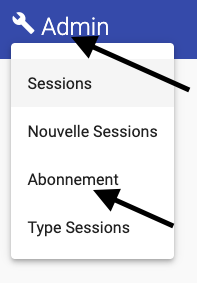
\includegraphics[width=0.4\textwidth,center]{Figures/us15-1}
	\caption{Menu de l'administrateur}
\end{figure}

\vspace{\baselineskip}
\begin{figure}[h]
	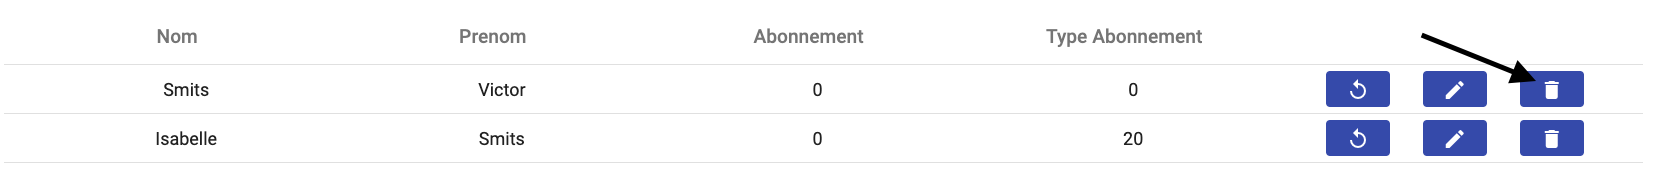
\includegraphics[width=\textwidth,center]{Figures/us15-2}
	\caption{Bouton de suppression de l'utilisateur}
\end{figure}

\vspace{\baselineskip}
\begin{figure}[h]
	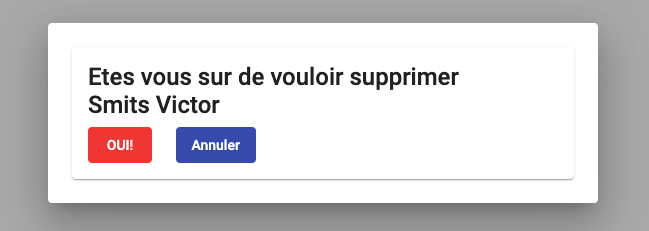
\includegraphics[width=0.5\textwidth,center]{Figures/us15-3}
	\caption{Fenêtre de confirmation de suppression}
\end{figure}

\subsubsection{Scripts concernés}
	\begin{itemize}
		\item \Href{https://github.com/victorsmits/Aquabike/blob/master/backend/src/Controller/API/AbonnementControllerApi.php}{AbonnementControllerApi.php}
		\item \Href{https://github.com/victorsmits/Aquabike/blob/master/backend/src/Entity/Person.php}{Person.php}
		\item \Href{https://github.com/victorsmits/Aquabike/blob/master/frontend/src/app/type-session/del-abo.component.ts}{del-abo.component.ts}
		\item \Href{https://github.com/victorsmits/Aquabike/blob/master/frontend/src/app/type-session/del-abo.component.html}{del-abo.component.html}
	\end{itemize}

	
	\newpage
	\subsection{En tant qu'administrateur, je dois pouvoir générer les sessions pour un nombre d'année}
		\begin{enumerate}
	\item L'administrateur se connecte au site avec ses identifiants. 
	\item Un nouveau bouton de navigation apparait dans la barre de navigation. 
	\item L'administrateur clique sur le bouton \textit{Admin}
	\item Il sélectionne \textit{Nouvelle session} dans le menu déroulant. 
	\item L'administrateur atterrit sur la page de création de session. 
	\item Il clique sur \textit{Génération auto}
	\item Un formulaire lui demandant sur combien d'années et le type de session il souhaite générer apparait.
	\item Il sélectionne les types de session qu'il souhaite générer.
	\item Il indique le nombre d'années voulus
	\item Il clique sur \textit{Je confirme la génération} 
\end{enumerate}

\vspace{\baselineskip}
\begin{figure}[h]
	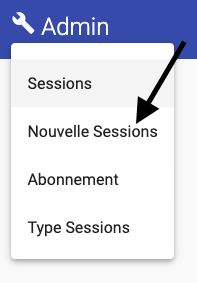
\includegraphics[width=0.4\textwidth,center]{Figures/us16-1}
	\caption{Menu de l'administrateur}
\end{figure}

\newpage
\begin{figure}[h]
	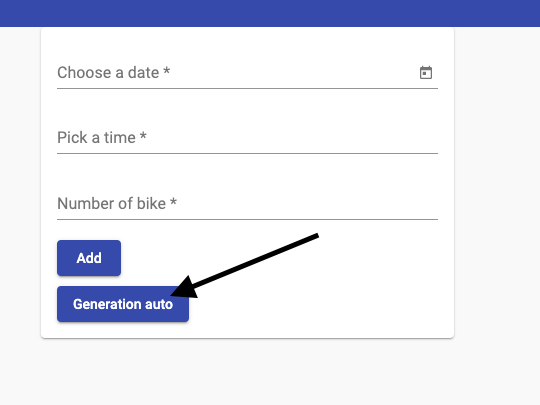
\includegraphics[width=0.4\textwidth,center]{Figures/us16-2}
	\caption{Bouton de génération automatique}
\end{figure}

\vspace{\baselineskip}
\begin{figure}[h]
	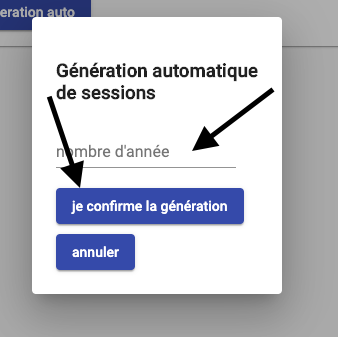
\includegraphics[width=0.3\textwidth,center]{Figures/us16-3}
	\caption{Formulaire pour la génération automatique de sessions}
\end{figure}


\subsubsection{Gestion des erreurs}
	\begin{itemize}
		\item La génération automatique suppose que tous les types de session on été préalablement configurés. Si ce n'est pas le cas, une erreur apparaitra à la confirmation.
		\item Si une erreur se crée durant la génération, elle est interrompue et un message d'erreur est affiché à l'administrateur.
	\end{itemize}
	
\newpage
\subsubsection{Diagramme de séquence}
	\begin{figure}[h]
		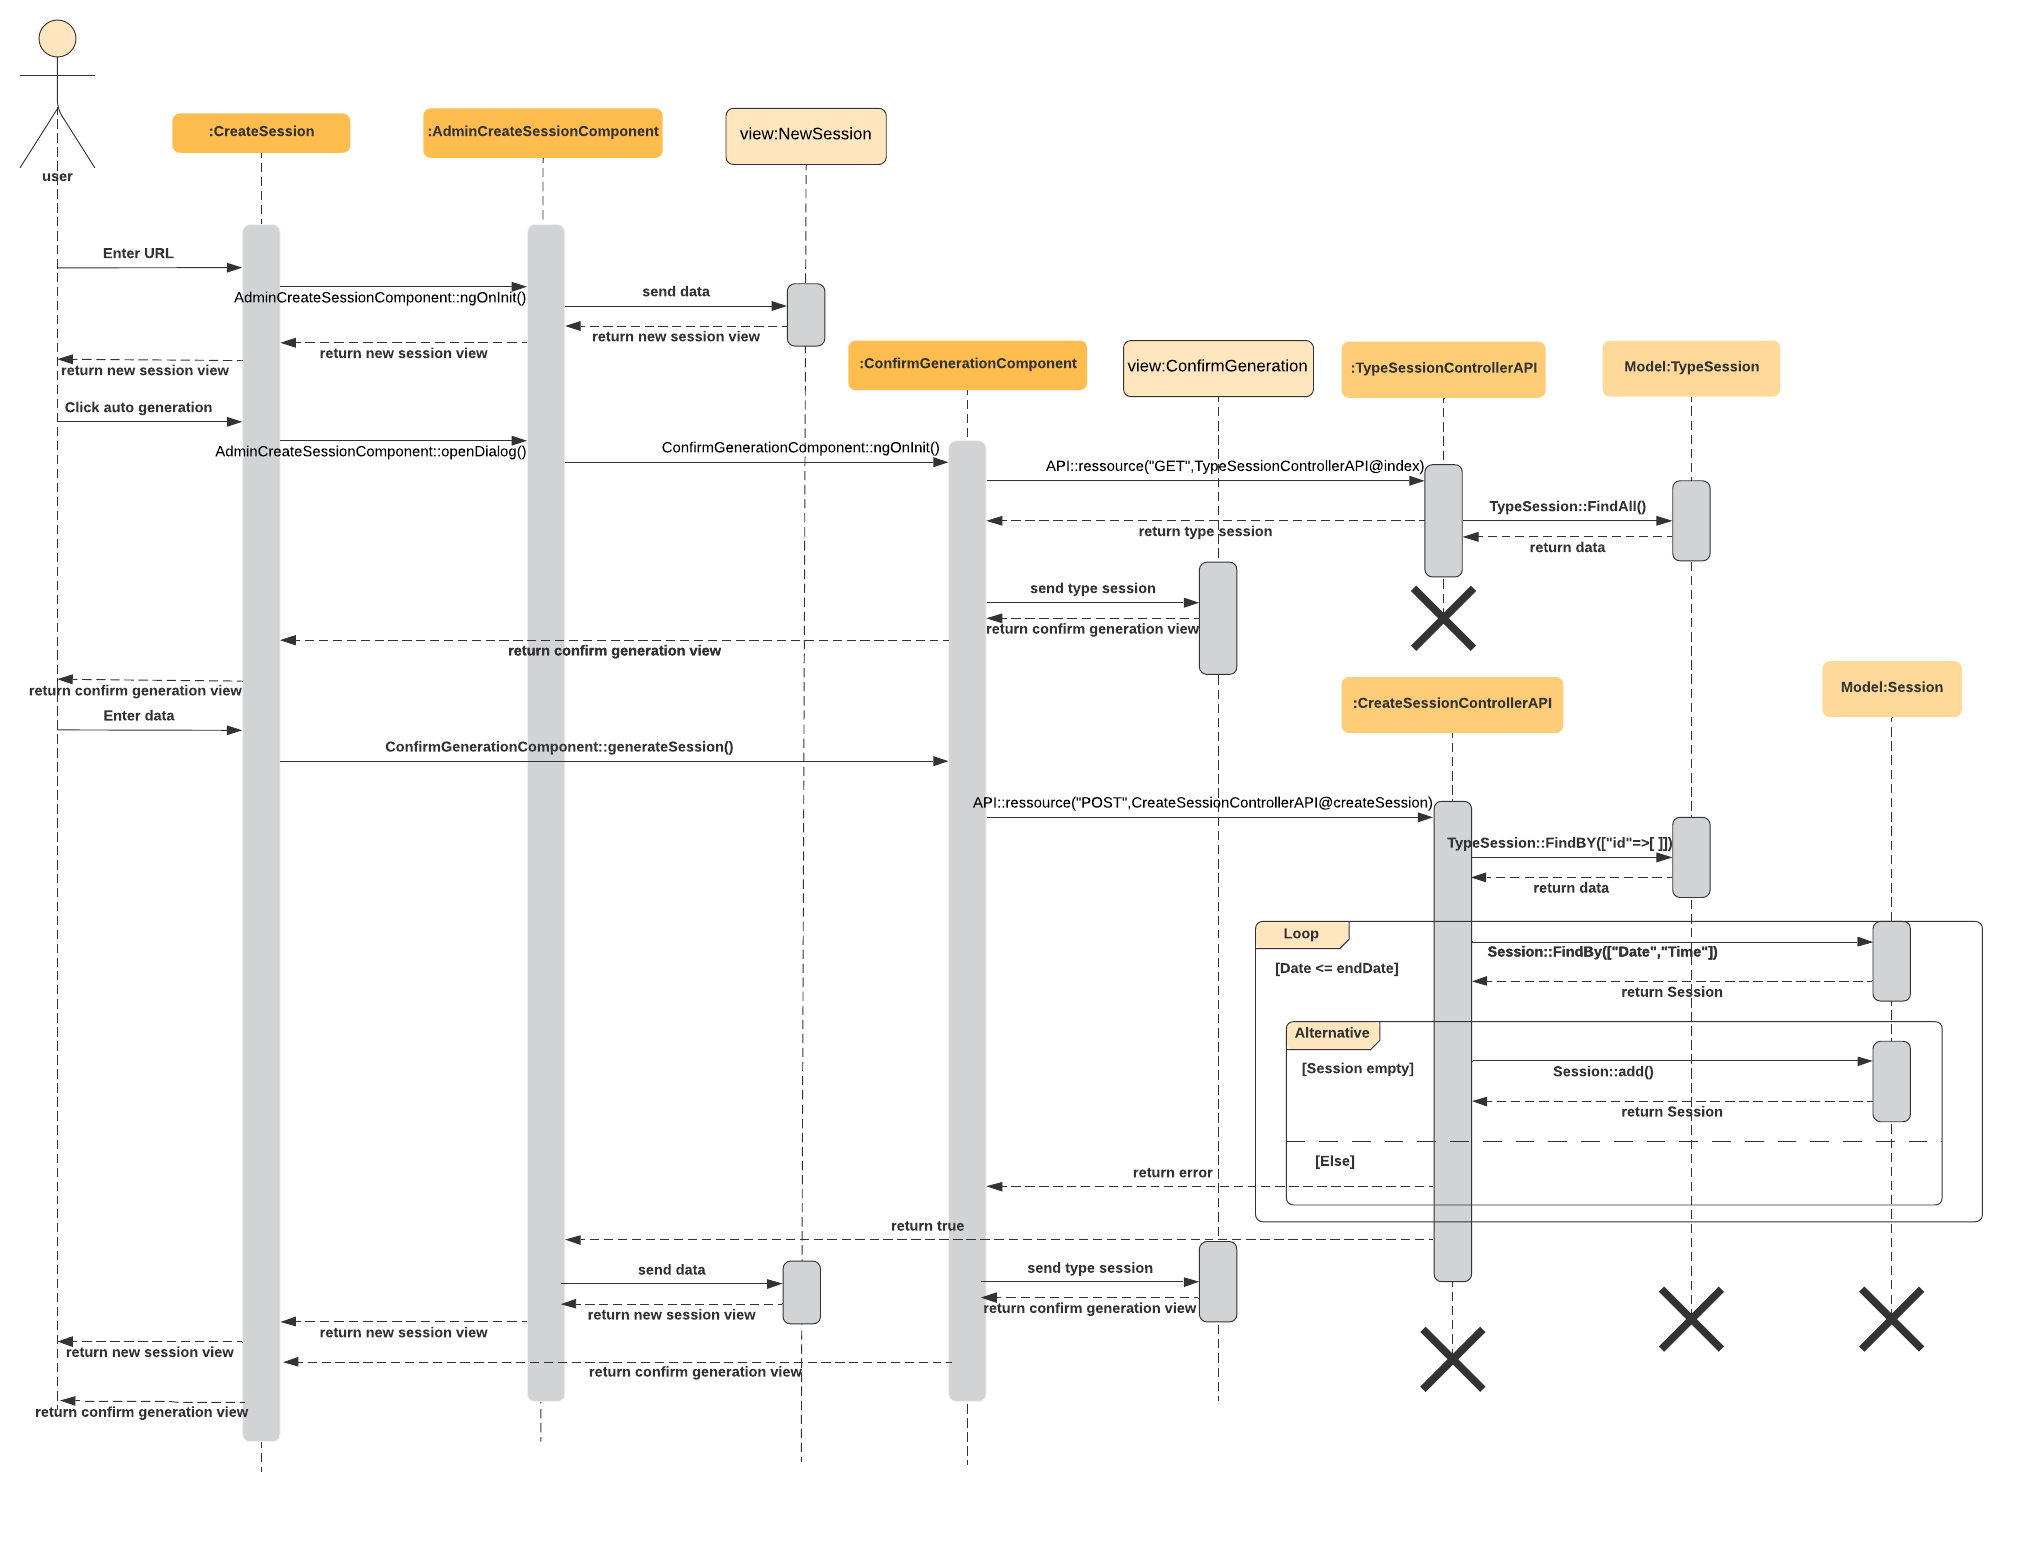
\includegraphics[width=\textwidth,center]{Diagramme/sequence-us16}
		\caption{Diagramme de séquence de la génération automatique de session}
	\end{figure}
	

\subsubsection{Scripts concernés}
	\begin{itemize}
		\item \Href{https://github.com/victorsmits/Aquabike/blob/master/backend/src/Entity/Session.php}{Session.php}
		\item \Href{https://github.com/victorsmits/Aquabike/blob/master/backend/src/Controller/API/CreateSessionControllerApi.php}{CreateSessionControllerApi.php}
		\item \Href{https://github.com/victorsmits/Aquabike/blob/master/frontend/src/app/admin-create-session/admin-create-session.component.ts}{admin-create-session.component.ts}
		\item \Href{https://github.com/victorsmits/Aquabike/blob/master/frontend/src/app/admin-create-session/admin-create-session.component.html}{admin-create-session.component.html}
	\end{itemize}

\newpage
\section{User Stories compatible Symfony-Angular}
	
	\subsection{En tant qu’utilisateur, je dois pouvoir me connecter sur le site}
		\subsubsection{Différences}
	\begin{itemize}
		\item Réalisation d'une requête POST via l'api REST permettant d'effectuer l'authentification dans le backend. 
		\item Différences au niveau de l'aspect graphique de la page de connection. 
		\item Connection via l'adresse Email et non le nom d'utilisateur. 
		\item Redirection automatique de l'utilisateur vers la page de connection lors de l'accès au site si l'utilisateur n'est pas connecté.
		\item Utilisation d'un LoginAuthenticator afin de pouvoir authentifier l'utilisateur dans le backend. 
		\item Utilisation de coockies pour préserver les informations de l'utilisateur. 
	\end{itemize}

\newpage
\subsubsection{Diagramme de séquence}
	\begin{figure*}[h!]
		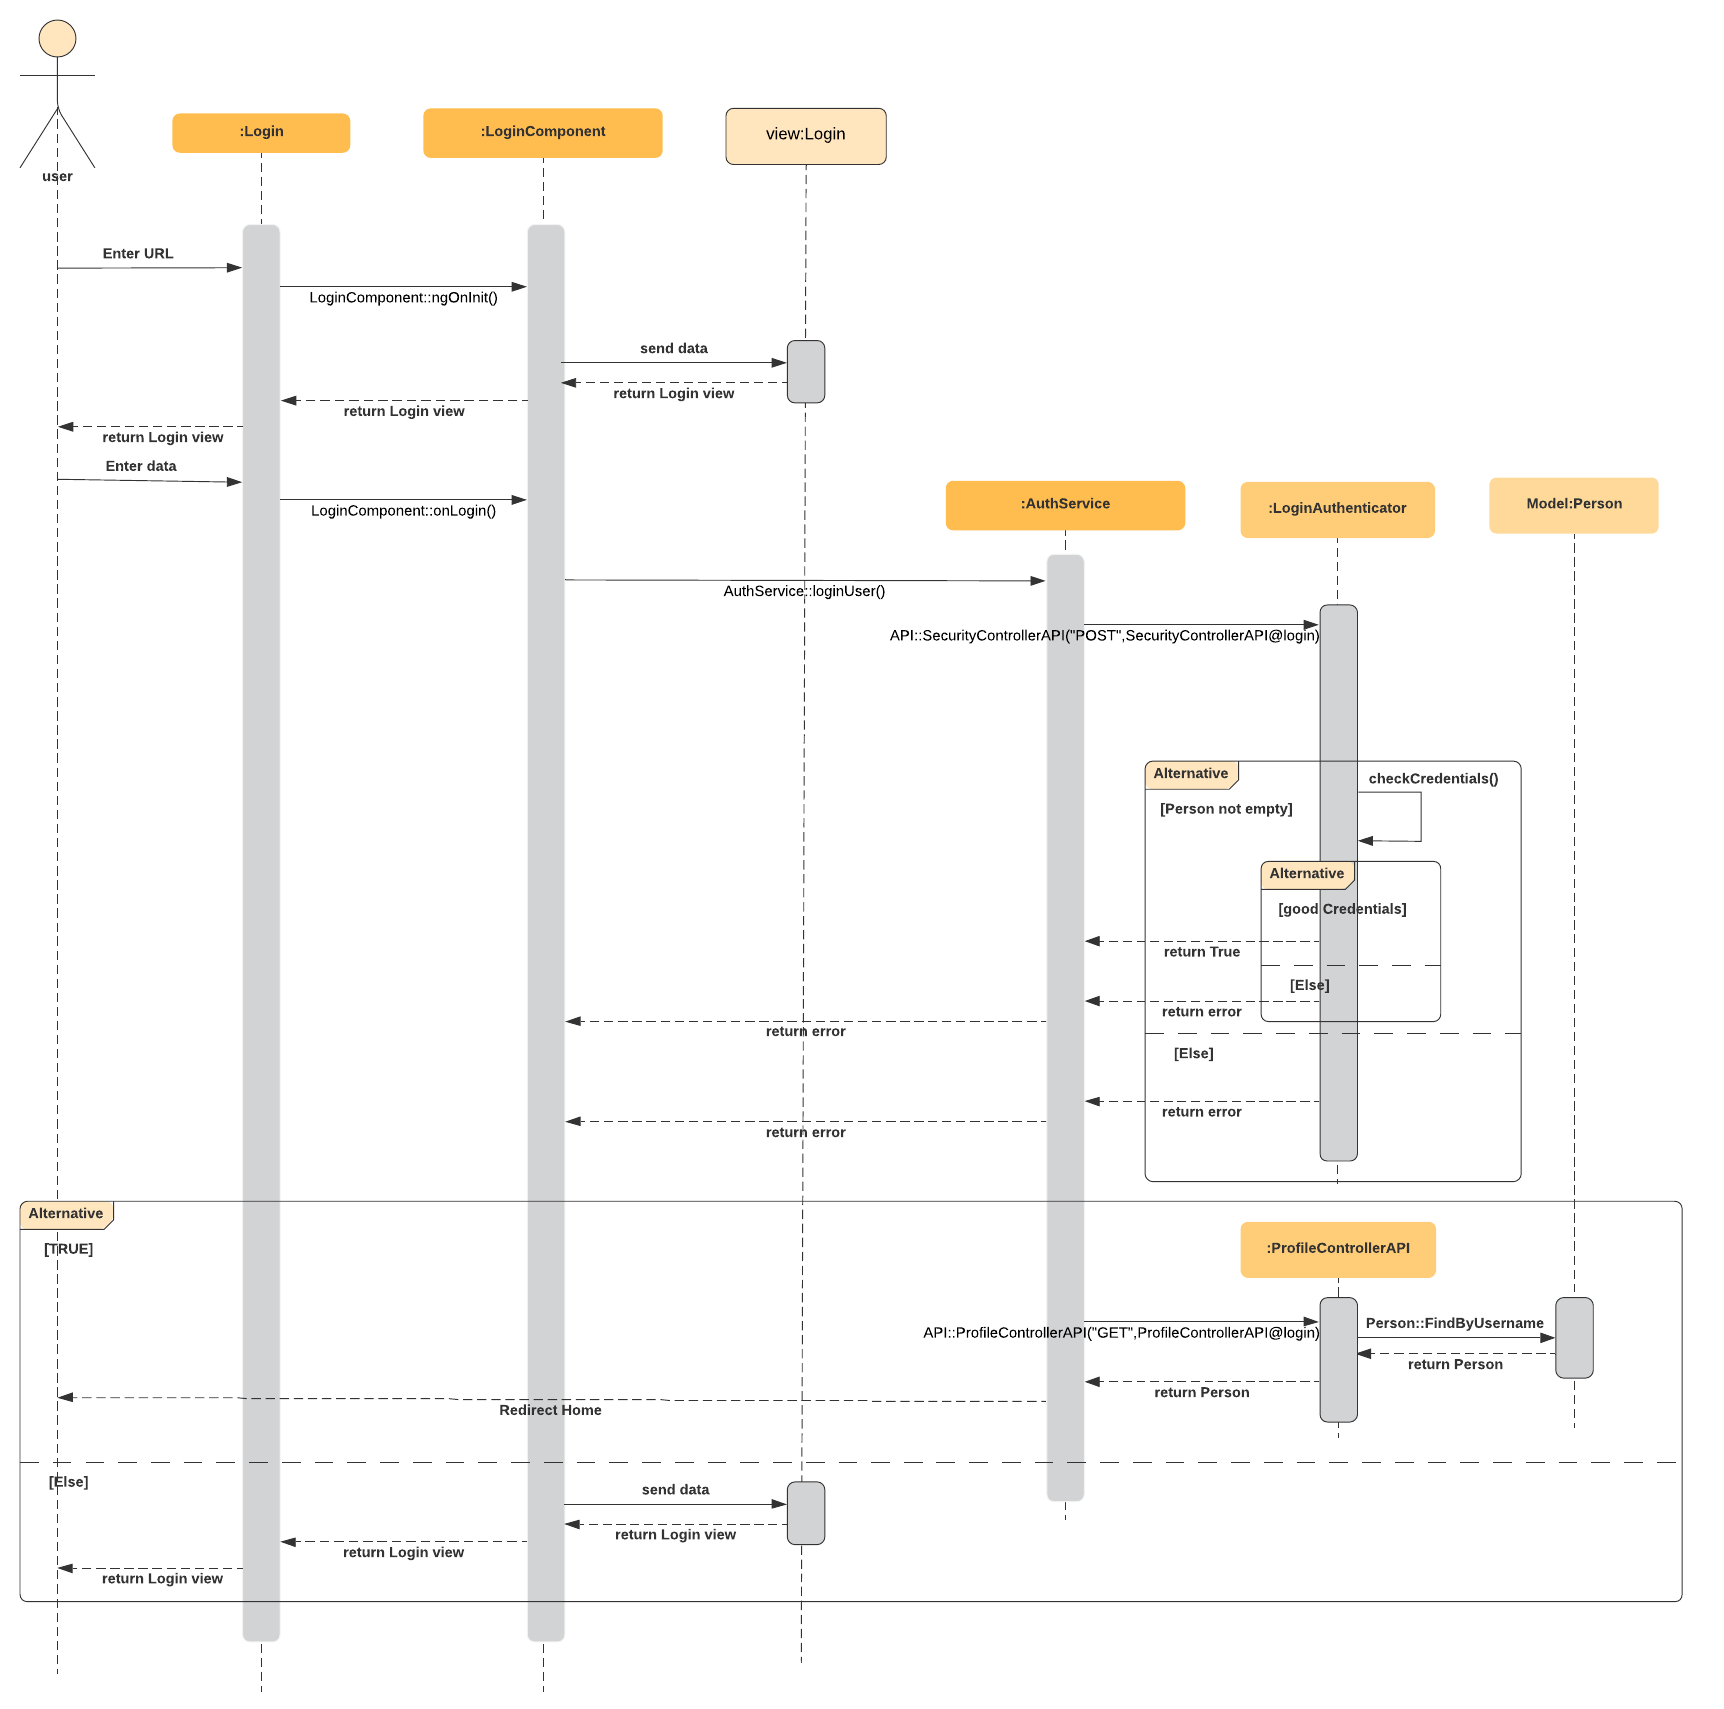
\includegraphics[width =\textwidth,center]{Diagramme/sequence-us0-angular}
		\caption{Diagramme de séquence de la connection d'un utilisateur}
	\end{figure*}

\newpage
\subsubsection{Scripts concernés}
	\begin{itemize}
		\item \Href{https://github.com/victorsmits/Aquabike/blob/master/frontend/src/app/service/api.service.ts}{api.service.ts}
		\item \Href{https://github.com/victorsmits/Aquabike/blob/master/frontend/src/app/service/auth.service.ts}{auth.service.ts}
		\item \Href{https://github.com/victorsmits/Aquabike/blob/master/backend/src/Controller/API/SecurityControllerAPI.php}{SecurityControllerAPI.php}
		\item \Href{https://github.com/victorsmits/Aquabike/blob/master/backend/src/Controller/API/ProfileControllerAPI.php}{ProfileControllerAPI.php}
		\item \Href{https://github.com/victorsmits/Aquabike/blob/master/frontend/src/app/login/login.component.ts}{login.component.ts}
		\item \Href{https://github.com/victorsmits/Aquabike/blob/master/frontend/src/app/login/login.component.html}{login.component.html}
		\item \Href{https://github.com/victorsmits/Aquabike/blob/master/backend/src/Entity/Person.php}{Person.php}
	\end{itemize}
	
	\newpage
	\subsection{En tant qu’utilisateur, je dois pouvoir me créer un compte sur le site}
		\begin{figure}[h]
	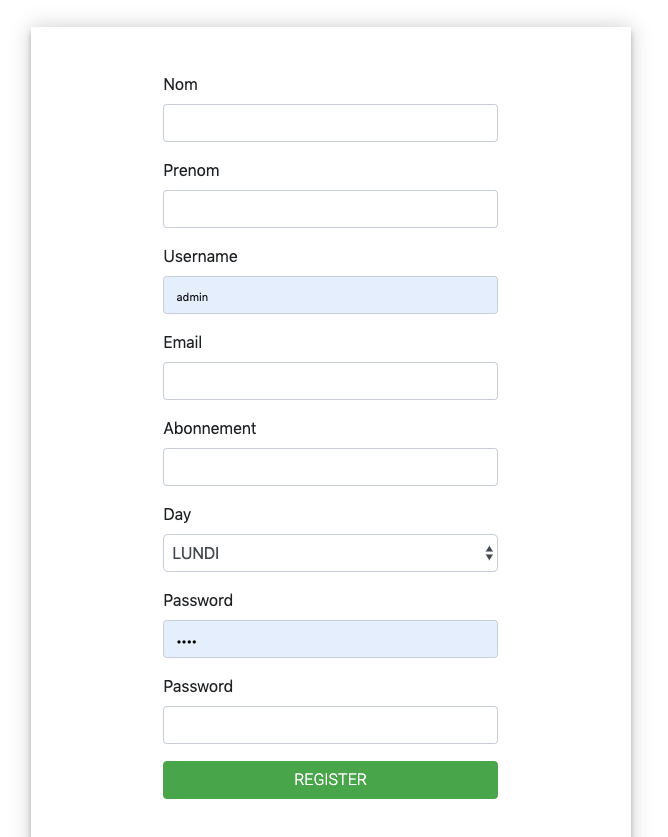
\includegraphics[width=0.5\textwidth,center]{Figures/us1-1}
	\caption{Formulaire d'inscription}
\end{figure}

\vspace{\baselineskip}
\begin{enumerate}
	\item L'utilisateur rentre ses information dans le formulaire. 
	\item L'utilisateur sélectionne le type de session à laquelle il est inscrit. 
	\item L'utilisateur clique sur \textit{Register} et attend la redirection. 
\end{enumerate}

\newpage
\subsubsection{Gestion des erreurs et sécurité}
	\paragraph{}
		\begin{itemize}
			\item L'utilisateur doit remplir tous les champs. Si un champ est manquant, une erreur apparaitra. 
			\item Le nom d'utilisateur et l'adresse Email sont uniques dans le système, s'il entre un Email ou nom d'utilisateur déjà existant, une erreur lui dira de corriger.
			\item L'utilisateur doit confirmer son mot de passe, si les mots de passe sont différents ou plus petits que 6 charactères il y aura un message d'erreur.
		\end{itemize}
		
\subsubsection{Diagramme de séquence}
	\begin{figure}[h]
		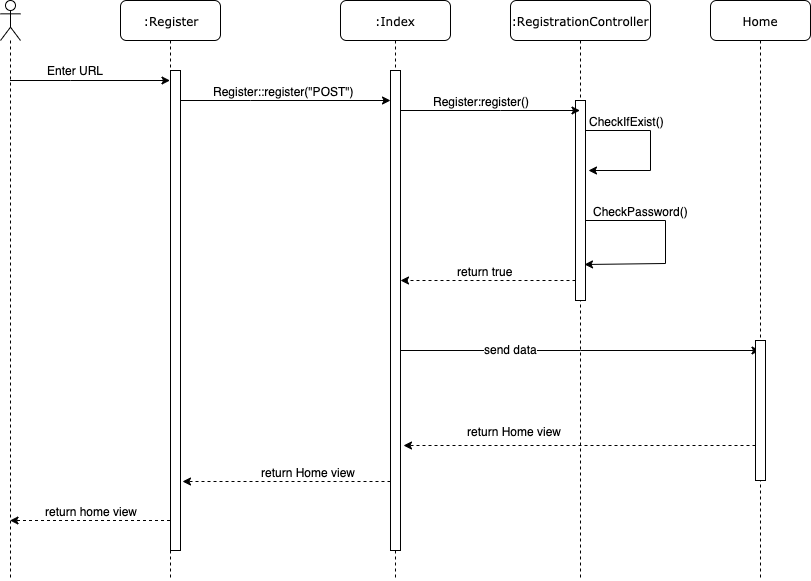
\includegraphics[width=0.8\textwidth,center]{Diagramme/sequence-us1}
		\caption{Diagramme de séquence de l'enregistrement d'un nouvelle utilisateur. }
	\end{figure}
	
	
\subsubsection{Scripts concernés}
	\begin{itemize}
		\item \Href{https://github.com/victorsmits/Aquabike/blob/master/backend/src/Controller/RegistrationController.php}{RegistrationController.php}
		\item \Href{https://github.com/victorsmits/Aquabike/blob/master/backend/templates/registration/register.html.twig}{register.html.twig}
		\item \Href{https://github.com/victorsmits/Aquabike/blob/master/backend/src/Entity/Person.php}{Person.php}
	\end{itemize}

	\vspace{\baselineskip}
	\subsection{En tant qu'utilisateur, je dois pouvoir sélectionner le mois et l'année pour afficher les sessions qui m'intéresse}
		\begin{figure*}[h]
	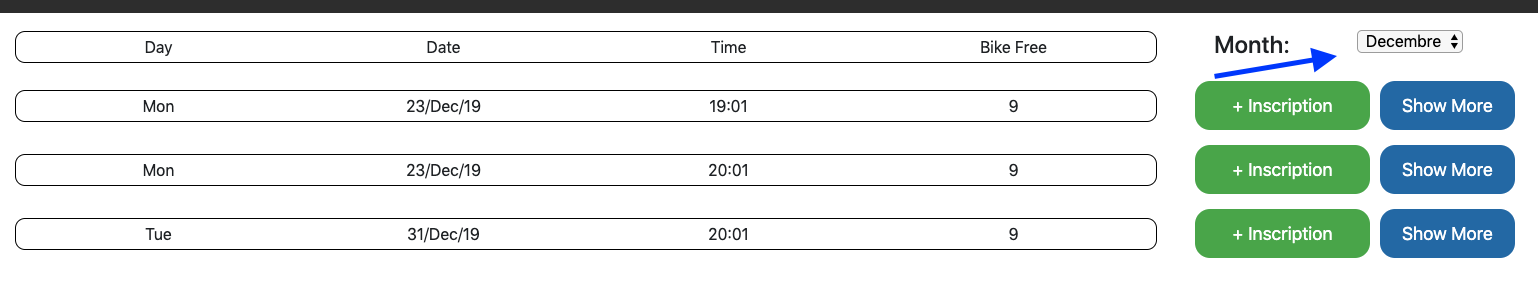
\includegraphics[width = 0.8\textwidth,center]{Figures/us2-1}
	\caption{selection du mois et de l'année}
\end{figure*}

\begin{enumerate}
	\item L'utilisateur choisit le mois et l'année. 
	\item la liste se rafraîchis afin de correspondre à la selection
\end{enumerate}
	
	\vspace{\baselineskip}
	\subsection{En tant qu’utilisateur, je dois pouvoir m’inscrire à une session un certain jour}
		\begin{figure*}[!h]
	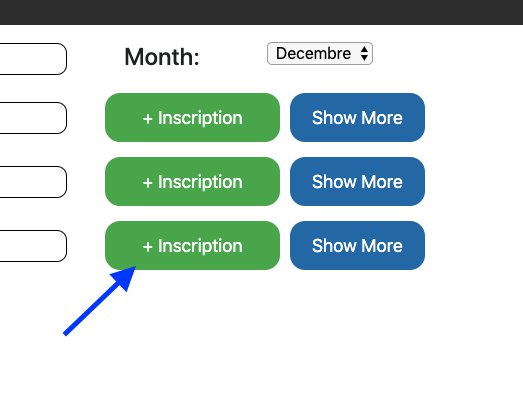
\includegraphics[width=0.5\textwidth,center]{Figures/us3-1}
	\caption{bouton d'inscritption}
\end{figure*}

\begin{enumerate}
	\item l'utilisateur choisit la session correspondant à sa demande.
	\item l'utilisateur clique sur le bouton  \textit{+ Inscription}
\end{enumerate}

\subsubsection{Gestion des erreurs}
	\begin{itemize}
		\item Si l'utilisateur ne possède plus d'abonnement, une erreur sera affichée lui signalant le problème. 
		\item Si la session est complète un message d'erreur sera affiché. 
	\end{itemize}
	
\subsubsection{Scripts concerné}
	\begin{itemize}
		\item \Href{https://github.com/victorsmits/Aquabike/blob/master/Symfony-Twig/src/Controller/MonthController.php}{MonthController.php}
		\item \Href{https://github.com/victorsmits/Aquabike/blob/master/Symfony-Twig/templates/month/month.html.twig}{month.html.twig}
		\item \Href{https://github.com/victorsmits/Aquabike/blob/master/Symfony-Twig/src/Entity/Session.php}{Session.php}
	\end{itemize}

	\vspace{\baselineskip}
	\subsection{En tant qu’utilisateur, je dois pouvoir être inscrit automatiquement à une session}
		\subsubsection{Différences}
	\begin{itemize}
		\item Réalisation de l'inscription automatique au session lors de l'enregistrement de l'utilisateurs. 
		\item Utilisation de type de session afin de facilité et de multiplier le choix des abonnements possible. 
		\item Possibilité pour un utilisateur de s'inscrire à plus de un type de session par semaine. 
		\item Sélection du type de session parmi une liste. 
	\end{itemize}

	\begin{figure*}[h!]
		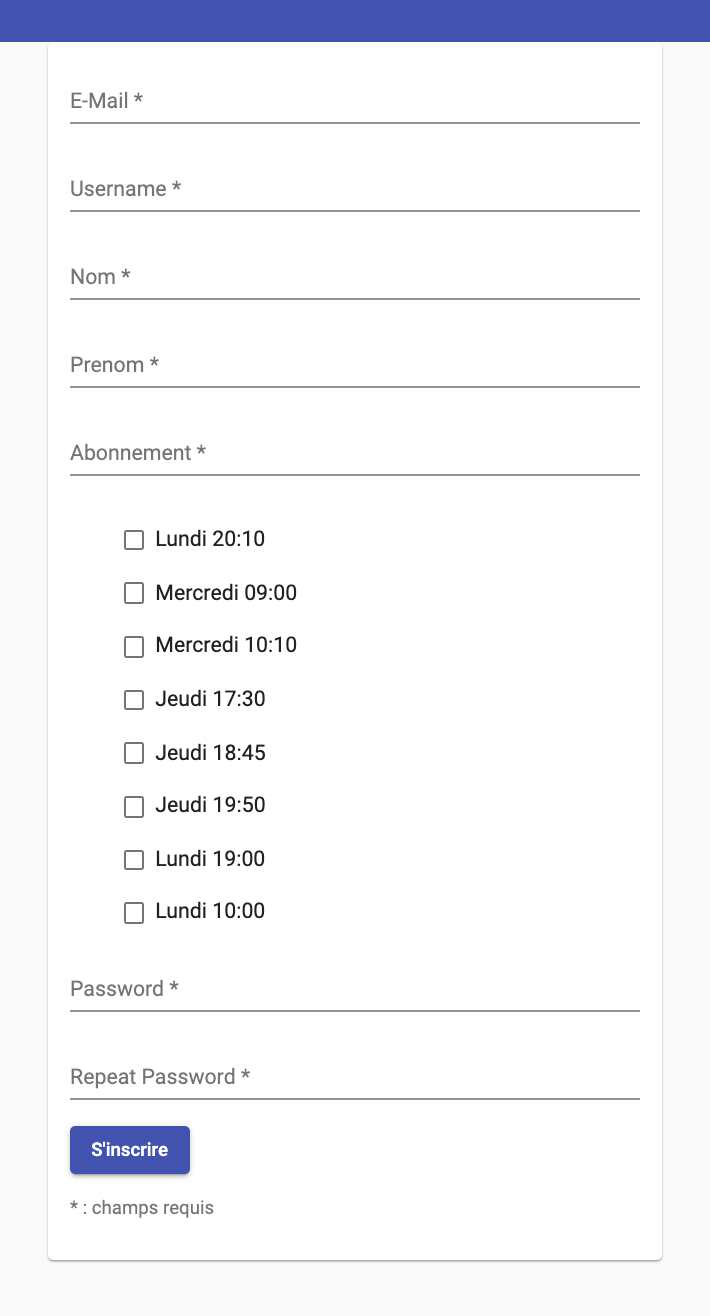
\includegraphics[width = 0.5\textwidth,center]{Figures/us4-1-angular}
		\caption{Formulaire d'inscription version angular}
	\end{figure*}
	
	
\newpage
\subsubsection{Diagramme de séquence}
	\begin{figure}[h]
		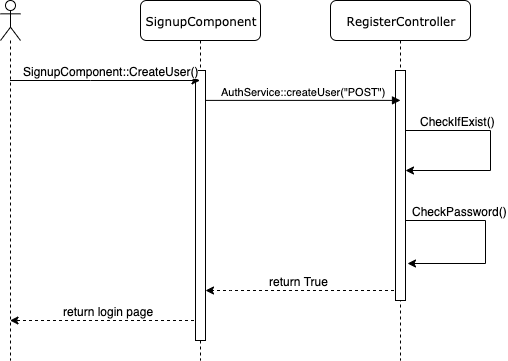
\includegraphics[width=\textwidth,center]{Diagramme/sequence-us1-angular}
		\caption{Diagramme de séquence de l'inscription automatique d'un utilisateur. }
	\end{figure}

\vspace{\baselineskip}
\subsubsection{Script concernés}
	\begin{itemize}
		\item \Href{https://github.com/victorsmits/Aquabike/blob/master/frontend/src/app/service/auth.service.ts}{auth.service.ts}
		\item \Href{https://github.com/victorsmits/Aquabike/blob/master/backend/src/Controller/API/SecurityControllerAPI.php}{SecurityControllerAPI.php}
		\item \Href{https://github.com/victorsmits/Aquabike/blob/master/backend/src/Entity/TypeSession.php}{TypeSession.php}
		\item \Href{https://github.com/victorsmits/Aquabike/blob/master/backend/src/Entity/Session.php}{Session.php}
		\item \Href{https://github.com/victorsmits/Aquabike/blob/master/backend/src/Entity/Inscription.php}{Inscription.php}
		\item \Href{https://github.com/victorsmits/Aquabike/blob/master/backend/src/Entity/Person.php}{Person.php}
		\item \Href{https://github.com/victorsmits/Aquabike/blob/master/frontend/src/app/signup/signup.component.ts}{signup.component.ts}
		\item \Href{https://github.com/victorsmits/Aquabike/blob/master/frontend/src/app/signup/signup.component.html}{signup.component.html}
	\end{itemize}
	
	\newpage
	\subsection{En tant qu’utilisateur, je dois pouvoir me désinscrire à une session}
		\begin{figure*}[h]
	\includegraphics[width=0.5\textwidth,center]{Figures/us5-1}
	\caption{Bouton de désinscription à une session}
\end{figure*}

\begin{enumerate}
	\item L'utilisateur trouve la session qui l'interesse.
	\item Le check vert indique qu'il est inscrit.
	\item Il clique sur le bouton.
\end{enumerate}

\vspace{\baselineskip}
\subsubsection{Script concernés}
	\begin{itemize}
		\item \href{https://github.com/victorsmits/Aquabike/blob/master/backend/src/Controller/MonthController.php}{MonthController.php}
		\item \href{https://github.com/victorsmits/Aquabike/blob/master/backend/templates/registration/month.html.twig}{month.html.twig}
		\item \href{https://github.com/victorsmits/Aquabike/blob/master/backend/src/Entity/Person.php}{Person.php}
		\item \href{https://github.com/victorsmits/Aquabike/blob/master/backend/src/Entity/Inscription.php}{Inscription.php}
	\end{itemize}

	\vspace{\baselineskip}
	\subsection{En tant qu’utilisateur, je dois pouvoir voir qui est inscrit pour chaque session}
		\vspace{\baselineskip}
\begin{figure}[h]
	\includegraphics[width=0.9\textwidth,center]{Figures/us6-1}
	\caption{Bouton d'affichage}
\end{figure}

\begin{figure}[h]
	\includegraphics[width=0.5\textwidth,center]{Figures/us6-2}
	\caption{Liste Participant(e)s}
\end{figure}

\begin{enumerate}
	\item L'utilisateur trouve la session qui l'intéresse. 
	\item L'utilisateur clique sur le bouton information dans la colonne \textit{Liste Participant(e)s}. 
	\item Un tableau s'affiche avec la liste des inscrit(e)s. 
\end{enumerate}
	
	\newpage
	\subsection{En tant qu’utilisateur, je veux pouvoir voir dynamiquement le nombre de séance qui reste dans mon abonnement}
		\begin{enumerate}
	\item L'utilisateur clique sur son nom dans la bar de navigation.
	\item L'utilisateur est redirigé vers sa page de profil. 
	\item L'utilisateur retrouve l'information dans le cadre afficher sur la page.
\end{enumerate}

\vspace{\baselineskip}
\begin{figure}[h]
	\includegraphics[width=0.5\textwidth,center]{Figures/us7-1}
	\caption{Bouton de navigation vers le profil}
\end{figure}

\vspace{\baselineskip}
\begin{figure}[h]
	\includegraphics[width=0.9\textwidth,center]{Figures/us7-2}
	\caption{Nombre de séance restante dans l'abonnement}
\end{figure}


\vspace{\baselineskip}
\subsubsection{Script concernés}
	\begin{itemize}
		\item \Href{https://github.com/victorsmits/Aquabike/blob/master/backend/src/Controller/ProfileController.php}{ProfileController.php}
		\item \Href{https://github.com/victorsmits/Aquabike/blob/master/backend/templates/registration/profile.html.twig}{profile.html.twig}
		\item \Href{https://github.com/victorsmits/Aquabike/blob/master/backend/src/Entity/Person.php}{Person.php}
	\end{itemize}


	\newpage
	\subsection{En tant qu'utilisateur, je veux pouvoir modifier mon profile}
		\begin{enumerate}
	\item L'utilisateur clique sur son nom dans la bar de navigation.
	\item L'utilisateur clique sur \textit{Profil} dans le menu déroulant.
	\item L'utilisateur clique sur le bouton edit au dessus de son profil. 
	\item Une fenêtre apparait. 
	\item L'utilisateur rentre les information qu'il souhaite changer. 
	\item L'utilisateur confirm en cliquant sur \textit{ok}
\end{enumerate}

\vspace{\baselineskip}
\begin{figure}[h]
	\includegraphics[width=0.4\textwidth,center]{Figures/us7-1}
	\caption{Bouton de navigation vers le profil}
\end{figure}

\begin{figure}[h]
	\includegraphics[width=0.4\textwidth,center]{Figures/us8-1}
	\caption{Bouton de modification du profil}
\end{figure}

\newpage
\begin{figure}[h]
	\includegraphics[width=0.4\textwidth,center]{Figures/us8-2}
	\caption{Fenêtre de modification des données du profil}
\end{figure}

	\newpage
	\subsection{En tant qu’administrateur, je dois pouvoir annuler une session}
		\subsubsection{Différences}
	\begin{itemize}
		\item Modification graphique du bouton d'annulation de la session. 
	\end{itemize}

\vspace{\baselineskip}
\subsubsection{Scripts concernés}
	\begin{itemize}
		\item \Href{https://github.com/victorsmits/Aquabike/blob/master/frontend/src/app/service/api.service.ts}{api.service.ts}
		\item \Href{https://github.com/victorsmits/Aquabike/blob/master/backend/src/Controller/API/SessionAdministrationControllerApi.php}{SessionAdministrationControllerApi.php}
		\item \Href{https://github.com/victorsmits/Aquabike/blob/master/backend/src/Entity/Session.php}{Session.php}
		\item \Href{https://github.com/victorsmits/Aquabike/blob/master/frontend/src/app/admin-session/admin-session.component.ts}{admin-session.component.ts}
		\item \Href{https://github.com/victorsmits/Aquabike/blob/master/frontend/src/app/admin-session/admin-session.component.html}{admin-session.component.html}
	\end{itemize}

	\vspace{\baselineskip}
	\subsection{En tant qu'administrateur, je dois pouvoir créer une nouvelle session peut importe la date}
		\subsubsection{Différence}
	\begin{itemize}
		\item Modification graphique du formulaire de création de session. 
	\end{itemize}
	
\vspace{\baselineskip}
\subsubsection{Script concernés}
	\begin{itemize}
		\item \href{https://github.com/victorsmits/Aquabike/blob/master/frontend/src/app/service/api.service.ts}{api.service.ts}
		\item \href{https://github.com/victorsmits/Aquabike/blob/master/backend/src/Controller/API/CreateSessionControllerApi.php}{CreateSessionControllerApi.php}
		\item \href{https://github.com/victorsmits/Aquabike/blob/master/backend/src/Entity/Session.php}{Session.php}
		\item \href{https://github.com/victorsmits/Aquabike/blob/master/frontend/src/app/admin-create-session/admin-create-session.component.ts}{admin-create-session.component.ts}
		\item \href{https://github.com/victorsmits/Aquabike/blob/master/frontend/src/app/admin-create-session/admin-create-session.component.html}{admin-create-session.component.html}
	\end{itemize}

	\vspace{\baselineskip}
	\vspace{\baselineskip}
	\subsection{En tant qu'administrateur, je dois pouvoir gérer les abonnement des utilisateurs}
		\subsubsection{Différence}
	\begin{itemize}
		\item Modification graphique de l'affichage des utilisateurs enregistré dans le système. 
	\end{itemize}

\vspace{\baselineskip}
\subsubsection{Script concernés}
	\begin{itemize}
		\item \href{https://github.com/victorsmits/Aquabike/blob/master/frontend/src/app/service/api.service.ts}{api.service.ts}
		\item \href{https://github.com/victorsmits/Aquabike/blob/master/backend/src/Controller/API/AbonnementControllerApi.php}{AbonnementControllerApi.php}
		\item \href{https://github.com/victorsmits/Aquabike/blob/master/backend/src/Entity/Person.php}{Person.php}
		\item \href{https://github.com/victorsmits/Aquabike/blob/master/frontend/src/app/admin-abo/admin-abo.component.ts}{admin-abo.component.ts}
		\item \href{https://github.com/victorsmits/Aquabike/blob/master/frontend/src/app/admin-abo/admin-abo.component.html}{admin-abo.component.html}
	\end{itemize}


\chapter{Conclusion}
\label{chap:Conclusion}

	\vspace{\baselineskip}
	\section{Objectifs atteints et non atteints}
	\subsection{Compatibles Symfony-Twig et Symfony-Angular}
		\begin{center}
			\begin{tabularx}{\textwidth}{|Y|T{0.1\textwidth}|T{0.15\textwidth}|Y|}
				\hline
				User Stories & Priorité & Réalisation & Reste à faire \\
				\hline	
				En tant qu’utilisateur, je dois pouvoir me créer un compte sur le site & 2 & 100\% & \\
				\hline
				En tant qu'utilisateur, je dois pouvoir sélectionner le mois et l'année pour afficher les sessions qui m'intéressent & 2 & 80\% & Sélection de l'année dans la partie symfony-twig et affichage des messages d'erreur sur le site Angular. \\
				\hline
				En tant qu’utilisateur, je dois pouvoir m’inscrire à une session un certain jour & 1 & 90\% & Afficher le message d'erreur sur le site Angular.\\
				\hline
				En tant qu’utilisateur, je dois pouvoir être inscrit automatiquement à une session & 1 & 80\% & Effectuer la boucle d'inscription pour la partie Symfony-Twig.  \\
				\hline
				En tant qu’utilisateur, je dois pouvoir me désinscrire à une session & 1 & 90\% & Afficher le message d'erreur sur le site Angular.\\
				\hline
				En tant qu’utilisateur, je dois pouvoir voir qui est inscrit pour chaque session & 2 & 100\% & \\
				\hline
			\end{tabularx}
		\end{center}
	
	\newpage
	\begin{center}
		\begin{tabularx}{\linewidth}{|Y|T{0.1\textwidth}|T{0.15\textwidth}|Y|}
			\hline
			En tant qu’utilisateur, je veux pouvoir voir dynamiquement le nombre de séances qui restent dans mon abonnement & 2 & 100\% &\\
			\hline
			En tant qu'utilisateur, je veux pouvoir modifier mon profil & 1 & 100\% &\\
			\hline
			En tant qu'utilisateur, je veux pouvoir m'inscrire à une session uniquement si il me reste des scéances a disposition. & 2 & 100\% &\\
			\hline
			En tant qu’administrateur, je dois pouvoir annuler une session & 2 & 90\% & Afficher les messages d'erreur sur le site Angular. \\
			\hline
			En tant qu'administrateur, je dois pouvoir gérer les abonnements des utilisateurs & 2 & 100\% & \\
			\hline
			En tant qu'administrateur, je dois pouvoir créer une nouvelle session peu importe la date & 2 & 80\% & Affichage des erreurs sur Twig et vérification de l'existence de la session créée.\\
			\hline

		\end{tabularx}
	\end{center}
	
	\newpage
	\subsection{Compatibles Symfony-Angular uniquement}
		\begin{center}
			\begin{tabularx}{\linewidth}{|Y|T{0.1\textwidth}|T{0.15\textwidth}|Y|}
				\hline
				En tant qu'administrateur, je dois pouvoir générer les sessions pour un nombre d'années & 1 & 100\% & \\
				\hline
				En tant qu'administrateur, je dois pouvoir créer un type de session & 2 & 100\% & \\
				\hline
				En tant qu'administrateur, je veux pouvoir gérer les types de sessions disponibles pour l'inscription automatique & 2 & 100\% &\\
				\hline
				En tant qu'administrateur, je veux pouvoir modifier un type de session & 1 & 100\% &\\
				\hline
				En tant qu'administrateur, je veux pouvoir supprimer un type de session & 1 & 90\% & Afficher le message d'erreur sur le site Angular.\\
				\hline
				En tant qu'administrateur, je veux pouvoir supprimer un utilisateur du système & 1 & 90\% & Afficher le message d'erreur sur le site Angular.\\
				\hline
			\end{tabularx}
		\end{center}
		
\section{Pistes d'amélioration}
	\begin{itemize}
		\item Optimisation des requêtes de base de données.
		\item Nettoyage du code source (duplication, réorganisation, …).
		\item Amélioration/Finition de la responsivité du site.
		\item Triage des sessions reçues dans angular pour un affichage trié en fonction du jour et de l'heure.
		\item Renommage des clés des json envoyées au frontend.
		\item Renommage de certains champs de la base de données.
		\item Utilisation d'une base de données orienté graph.
		\item Lors de la creation d'une session, trouver un type de session compatible si existant, sinon mettre le paramètre à NULL. 
	\end{itemize}

\newpage
\chapter{Annexe}
	 \label{chap:Annexe}
	
	\vspace{\baselineskip}
	\section{Code source}
		\paragraph{}
			Retrouvez l'entièreté du code source sur le Github suivant : \href{https://github.com/victorsmits/Aquabike}{Aquabike}
			
\end{document}